% This is "sig-alternate.tex" V1.9 April 2009
% This file should be compiled with V2.4 of "sig-alternate.cls" April 2009
%https://preview.overleaf.com/public/xnxjwzrdnynz/images/847ede20267048b902ed3c91cbcfe6aed1f31b8a.jpeg
% This example file demonstrates the use of the 'sig-alternate.cls'
% V2.4 LaTeX2e document class file. It is for those submitting
% articles to ACM Conference Proceedings WHO DO NOT WISH TO
% STRICTLY ADHERE TO THE SIGS (PUBS-BOARD-ENDORSED) STYLE.
% The 'sig-alternate.cls' file will produce a similar-looking,
% albeit, 'tighter' paper resulting in, invariably, fewer pages.
%
% ----------------------------------------------------------------------------------------------------------------
% This .tex file (and associated .cls V2.4) produces:
%       1) The Permission Statement
%       2) The Conference (location) Info information
%       3) The Copyright Line with ACM data
%       4) NO page numbers
%
% as against the acm_proc_article-sp.cls file which
% DOES NOT produce 1) thru' 3) above.
%
% Using 'sig-alternate.cls' you have control, however, from within
% the source .tex file, over both the CopyrightYear
% (defaulted to 200X) and the ACM Copyright Data
% (defaulted to X-XXXXX-XX-X/XX/XX).
% e.g.
% \CopyrightYear{2007} will cause 2007 to appear in the copyright line.
% \crdata{0-12345-67-8/90/12} will cause 0-12345-67-8/90/12 to appear in the copyright line.
%
% ---------------------------------------------------------------------------------------------------------------
% This .tex source is an example which *does* use
% the .bib file (from which the .bbl file % is produced).
% REMEMBER HOWEVER: After having produced the .bbl file,
% and prior to final submission, you *NEED* to 'insert'
% your .bbl file into your source .tex file so as to provide
% ONE 'self-contained' source file.
%
% ================= IF YOU HAVE QUESTIONS =======================
% Questions regarding the SIGS styles, SIGS policies and
% procedures, Conferences etc. should be sent to
% Adrienne Griscti (griscti@acm.org)
%
% Technical questions _only_ to
% Gerald Murray (murray@hq.acm.org)
% ===============================================================
%
% For tracking purposes - this is V1.9 - April 2009

\documentclass{sig-alternate}
  \pdfpagewidth=8.5truein
  \pdfpageheight=11truein
\usepackage[hidelinks]{hyperref}
\usepackage{fancyvrb}
\usepackage{multicol}
\usepackage{subfig}
\usepackage{alphalph}
\renewcommand\thesubfigure{\alphalph{\value{subfigure}}}

\begin{document}
\title{Author Profiling from Personal Content Blogs}
%
% You need the command \numberofauthors to handle the 'placement
% and alignment' of the authors beneath the title.
%
% For aesthetic reasons, we recommend 'three authors at a time'
% i.e. three 'name/affiliation blocks' be placed beneath the title.
%
% NOTE: You are NOT restricted in how many 'rows' of
% "name/affiliations" may appear. We just ask that you restrict
% the number of 'columns' to three.
%
% Because of the available 'opening page real-estate'
% we ask you to refrain from putting more than six authors
% (two rows with three columns) beneath the article title.
% More than six makes the first-page appear very cluttered indeed.
%
% Use the \alignauthor commands to handle the names
% and affiliations for an 'aesthetic maximum' of six authors.
% Add names, affiliations, addresses for
% the seventh etc. author(s) as the argument for the
% \additionalauthors command.
% These 'additional authors' will be output/set for you
% without further effort on your part as the last section in
% the body of your article BEFORE References or any Appendices.

\numberofauthors{5} %  in this sample file, there are a *total*
% of EIGHT authors. SIX appear on the 'first-page' (for formatting
% reasons) and the remaining two appear in the \additionalauthors section.
%
\author{
% You can go ahead and credit any number of authors here,
% e.g. one 'row of three' or two rows (consisting of one row of three
% and a second row of one, two or three).
%
% The command \alignauthor (no curly braces needed) should
% precede each author name, affiliation/snail-mail address and
% e-mail address. Additionally, tag each line of
% affiliation/address with \affaddr, and tag the
% e-mail address with \email.
%
% 1st. author
\alignauthor Aayush Singhal\\
       \affaddr{12CS10002}
% 2nd. author
\alignauthor Aseem Patni\\
       \affaddr{12CS10008}
% 3rd. author
\alignauthor Soham Dan\\
       \affaddr{12CS10059}\\
\and
% 4th. author
\alignauthor Bhushan Kulkarni\\
       \affaddr{12CS30016}
\alignauthor Pranay Yadav\\
       \affaddr{12CS30025}
% 6th. author
\alignauthor Shubham Saxena\\
       \affaddr{12CS30032}\\
\and 
\alignauthor Sruthi Warrier\\
       \affaddr{Mentor}
\alignauthor Anurag Verma\\
       \affaddr{Mentor}
\alignauthor Suman Kalyan Maity\\
       \affaddr{Mentor}\\
}
\date{30 July 2015}
\maketitle
\begin{abstract}
This project aims to predicting personally identifiable information (PII), such as age and gender of the author by extracting features from his/her personal content blog texts. We intend to define the state-of-the-art in the field and overcome the shortcomings of the prior works in the personality recognition tasks. This report is meant to share our progress so far and contains details about our future plans.
\end{abstract}

\keywords{Authorship Profiling, PII, Blogosphere, Natural Language Processing}

\section{Introduction}
Though the enormous impact of social media on our daily life, we observe a lack of information about those who create the contents. In this regard, author profiling tries to determine the gender, age, native language or personality type of authors by analyzing their published texts. In this study, we focus on building a system to identify only the gender and age of the authors. Other authorship details will be a part of the future work in this area. Author profiling is of growing importance: E.g., from a marketing viewpoint, companies may be interested in knowing the demographics of their target group in order to achieve a better market segmentation; from a forensic viewpoint, determining the linguistic profile of a person who wrote a "suspicious text" may provide valuable background information.\\\\
This study is targeted towards partial fulfillment of requirements for \textit{CS60057: Speech \& Natural Language Processing} during Fall 2015, under the guidance of Prof. Pawan Goyal.\\\\
The remainder of this paper is organized as follows. Section 2 describes the corpus, Section 3 covers the proposed approach, Section 4 presents the results obtained so far, Section 5 discusses the evaluation measures, Section 6 contains details about the future work-plan, Section 7 enumerates the references and Section 8 concludes by listing the work done by the individual team-mates.
\newpage
\section{Data-set}
\subsection{Corpus}
We have used the following two corpora for this study:
\begin{itemize}
\item \textbf{Blog Authorship Corpus \cite{koppel1}}\\
The Blog Authorship Corpus consists of the collected posts of 19,320 bloggers gathered from blogger.com in August 2004. The corpus incorporates a total of 681,288 posts and over 140 million words or approximately 35 posts and 7250 words per person. All bloggers included in the corpus fall into one of three age groups --- "10s" [13-17], "20s" [23-27], "30s" [33-47].
For each age group there are an equal number of male and female bloggers.   
\item \textbf{PAN'14 Corpus}\\
As a part of the Author Profiling Shared Task in PAN '14, this corpus was made available for use during the competition. This data-set originally consists of blog posts, tweets and social media texts written in both English and Spanish as well as hotel reviews in English. We have considered only the subset which contains blog posts. All bloggers included in the corpus fall into one of these age groups: [18-24], [25-34], [35-49], [50-64], [65-xx].
The corpus incorporates a total of 2278 posts, 148 authors or on an average 15 blogs per author. 
\end{itemize}
We split ourselves into two groups, one for extracting features from the Blog Authorship Corpus (Pranay, Shubham \& Soham) and the other from the PAN '14 Corpus (Aayush, Aseem \& Bhushan).  
\subsection{Data Cleaning \& Extraction}
\begin{itemize}
\item \textbf{Blog Authorship Corpus}\\
The corpus contains 19,320 XML files, each pertaining to a particular author, identified by the unique file-names. Each XML file contains date when the blog was posted followed by the post itself. All the HTML links in the post are replaced by a unique tag \textit{'urlLink'} to mark their presence. We cleaned the data by discarding empty blog posts and ignoring posts which contain only HTML links and no text. We then exported this refined data to a JSON file, on which further analysis will be carried out.
\item \textbf{PAN '14 Corpus}\\
This corpus contains 148 XML files, each pertaining to a particular author. Each XML file contains the Author's unique ID and blogs written by the Author. The blog text is present in \texttt{CDATA} section. To parse this text, we wrote a regular expression to remove the HTML tags, translated HTML entities like \texttt{'\&amp;', '\&ldquo;'} to their usual textual counter-parts like '\&','"'. We then dumped this data as to a JSON file, on which further analysis will be carried out.
\end{itemize}


\section{Approach}
After obtaining the JSON files containing refined data from the both the corpora, we now start extracting features from this data-set. We shall be focusing our attention towards building two kinds of classifiers --- 1) Binary classifier for classification of gender and 2) Multi-label classifier for classification of age into predefined class labels. Later, we will also consider the possibility of predicting the age by fitting regression models, by working under the assumptions that --- 1) There are enough data points for the model to fit accurately and 2) Age behaves like a continuous variable. 

\subsection{Exhaustive Feature Set}
Different  people  tend  to  write  differently.  These  differences  occur  due  to  variations in the topics of interest and style of writing like word choices and grammar rules. For example, females tend to write more about wedding styles and male tends to write more
about technology and politics. Further females use more adverbs and adjectives while
writing compared to males. We considered these differences in the writing styles
and content of male and female bloggers of different ages. Overall we considered three
different types of features that are useful for distinguishing between different categories
--- content-based, style-based and semantic features. These are enumerated below:
\begin{itemize}
\item \textbf{Content-based Features} 

Male and female authors tend to speak about different topics,
so they will use different words. Thus content based features are important to distin-
guish between male and female bloggers

viz. \# of HTML links in the blog, \# of named entities used, \# of non-word errors, \# of discourse relations within the text, \# of quotations used in the text, \# of references to past or future within the text, \# of facts \& figures used, \# of times opinions are expressed, overall sentiment score of the blog, \# of words having character flooding (like 'hellooooo').

\item \textbf{Style-based Features} 

Features we used include distribution of POS tags, distribution of punctuation tag,s readability measure of the blog (SMOG, Flesch, Gunning Fog etc.), \# of co-references (usage of pronouns), average sentence length, usage of figures of speech by the author (like metaphor, alliteration). 
\item \textbf{Semantic Features}

We shall find a set of topics authors, belonging to a particular gender or age group, blog about. We shall also use Wikipedia concepts and category information to represent the document (blog) \cite{iiit-god}. These together will be used as semantic features, as explained in the following section.
\end{itemize}
These features will be extracted for both the corpora.
\subsection{Extracting Feature Vectors}
Methodology to extract feature vectors from the Blog Authorship Corpus is described below:
\begin{itemize}
\item Content-based Features:\\
1) \# of HTML links: count the occurrence of \textit{'urlLink'} in the body of the blog.\\
2) \# of named entities: Using Stanford NLTK APIs to tokenize blog text into sentences, perform POS Tagging and then extract named entities (NE) from the tagged sentences.\\
3) \# of non-word errors: Using Stanford NLTK's word corpus \texttt{nltk.corpus.words.words()} to keep a count of non-word errors in the blog.\\
4) \# of discourse relations within the text: Using a \href{https://github.com/ilija139/PDTB-Parser}{Java-based end-to-end PDTB-styled Discourse Parser} to identify implicit \& explicit discourse relations and keeping a count of each of them.\\
5) \# of quotations used in the text: Checking for occurrences of '"' in the blog text.\\
6) \# of references to past or future: Checking for occurrences of the following set of words and phrases - ['years ago','years from now','in the past','in future','once upon a time','\textasciicircum \textbackslash d\{4\}\$']. The last entry is a regex for detecting reference to a year.\\
7) \# of facts \& opinions used: Using SentiWordNet to assign score to each blog text; if this score is below 0.1, it is reported as 'fact', 'opinion' otherwise.\\
8) Overall Sentiment Score: Review of the PAN '14 Author Profiling Shared Task reveals that incorporating the overall sentiment score of the blog text yields no improvement in accuracy of the classifier. Hence, we shall not consider this feature in this study.
\item Style-based Features:\\
1) Distribution of POS tags: We use Stanford POS tagger to tag the sentences and collect total counts of all the POS tags for different age buckets \& gender. This count is then modeled as a random variable and a CDF is prepared which reports what is the probability that this random variable (say X) will be found to have a value less than or equal to the argument (say x).
\begin{align}
F_X(x) = P(X \leq x)
\end{align}
This CDF is prepared for all the age-buckets and both the gender separately.\\
2) Readability measure of the blog: We use Stanford NLTK's \texttt{punkt} module for assigning readability scores according to different metrics like ARI, Gunning Fog Index, SMOG Index etc. Similar to distribution of POS tags, we shall prepare CDF for the readability score as well.\\ 
3) Usage of Pronouns: Keeping a count of pronouns, used for referencing rather than directly nouns, for all the age-buckets and both the gender.\\
4) Average Sentence Length: We keep a average sentence length for the blogs authored by different age buckets and sexes.\\
5) Usage of Figures of Speech: To be decided.
\item Semantic Features:\\
1) LSA to identify topics a person usually blogs about: We use LSA technique to analyze relationships between a set of blogs written by a given author and the terms they contain by producing a set of concepts related to the blogs and terms. We will also try using simple Tf-Idf scores to identify topical words from the blogs authored by a single person, in order to get a set of topics he/she usually blogs about.\\
2) Wikipedia Categorization: We shall use Wikipedia concepts and category information to represent the document (blog) \cite{iiit-god}
\end{itemize}
\subsection{Feature Subset Selection (FS)}
Dimensionality reduction (DR) and Feature Subset Selection (FS) are two techniques for reducing the attribute space of a feature set. The main idea of FS is to remove redundant or irrelevant features from the data set as they can lead to a reduction of the classification accuracy and to an unnecessary increase of computational cost. The advantage of FS is that no information about the importance of single features is lost. For now, we will focus our attention on using FS over DR because DR can decrease the size of the attribute space strikingly. Another important disadvantage of DR is the fact that the linear combinations of the original features are usually not interpretable and the information about how much an original attribute contributes is often lost \cite{mit} .f possible, we might also try using DR technique (PCA) to our feature set and evaluate the improvement in the accuracy of the resulting classifier, if any.\\
There are three types of feature subset selection approaches:
\begin{itemize}
\item Filters:\\
Filters are classifier agnostic pre-selection methods which are independent of the later
applied machine learning algorithm. . Besides some statistical filtering methods like Fisher score or Pearson correlation, information gain is often used to find out
how well each single feature separates the given data set.\\
The overall entropy I of a given dataset S is defined as:
\begin{align}
I(S) := - \sum_{i=1}^{C} p_i log_2 p_i
\end{align}
where $C$ denotes the total number of classes and $p_i$ the portion of instances that belong to class $i$. The reduction in entropy or the information gain is computed for each attribute according to:
\begin{align}
IG(S,A) = I(S) - \sum_{v \in A} \frac{|S_{A,v}|}{|S|}I(S_{A,v})
\end{align}
where $v$ is a value of $A$ and $S_{A,v}$ is the set of instances where $A$ has value $v$.
\item Wrappers:\\
Wrappers are feedback methods which incorporate the ML algorithm in the FS process,
i.e. they rely on the performance of a specific classifier to evaluate the quality of a set of features. Wrapper methods search through the space of feature subsets and calculate
the estimated accuracy of a single learning algorithm for each feature that can be added
to or removed from the feature subset.
\end{itemize} 
We shall focus our attention towards using Filters to perform FS in this study.
\subsection{Building Classifiers \& Evaluation}
Having a reduced set of features, we shall now try building all types of classifiers available today --- Naive Bayes, SVMs, Logistic Regression, k-NN, Decision Trees etc., and evaluate their performance according to the following metrics:
\begin{itemize}
\item Precision
\begin{align}
P = \frac{TP}{TP+FP}
\end{align}
The percentage of positive predictions that are correct.
\item Recall
\begin{align}
R =  \frac{TP}{TP+FN}
\end{align}
The percentage of positive labeled instances that were predicted as positive.
\item Specificity
\begin{align}
S = \frac{TN}{TN+FP}
\end{align}
The percentage of negative labeled instances that were predicted as negative.
\item Accuracy
\begin{align}
A = \frac{TP+TN}{TP + TN + FP + FN}
\end{align}	The percentage of predictions that are correct.\\\\
If time permits, we shall also explore the possibility of modeling the prediction of age as a regression problem and try to improve the baseline established by \cite{cmu}. 
\end{itemize}
\section{Results So Far}
We have looked into influence of individual features in prediction of the age and gender. And because of high variance in these plots, it is clear that individual features, which we think are important distinguishing elements, don't play much role in the personality detection. We need to consider a combination of these in order to get something meaningful. We will next try to learn a classifier, that learns the weight given to each feature. This way we would be able to consider a combination of features and we'll also learn how much important a feature is in the required task.
\subsection{Blog Authorship Corpus}
Here goes the description about the plots obtained from the Blog Authorship Corpus.

\begin{figure*}
\subfloat[\# of Facts vs Age]{
  \label{fig:Total_scatter}%
  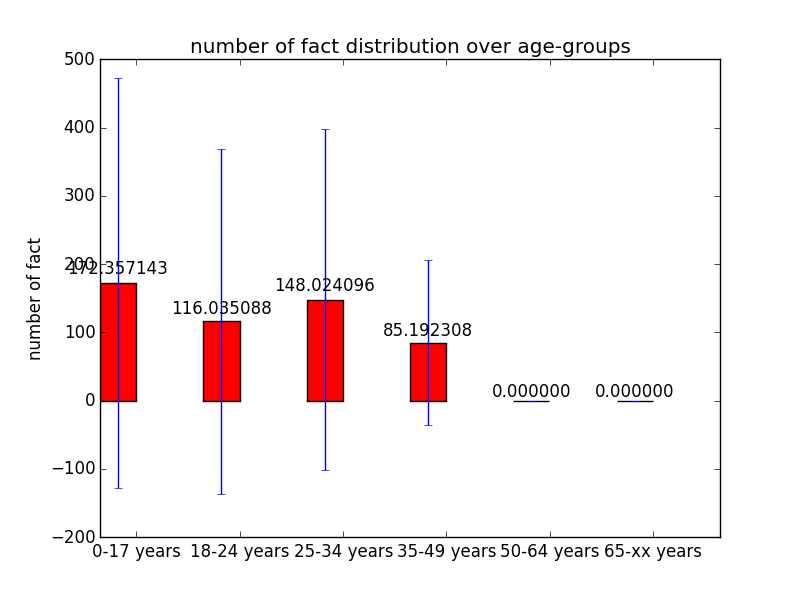
\includegraphics[width=0.5\textwidth]{koppel/age_numfact.png}%
}%
\hspace*{\fill}
\subfloat[\# of Opinions vs Age]{
  \label{fig:Num_scatter}%
  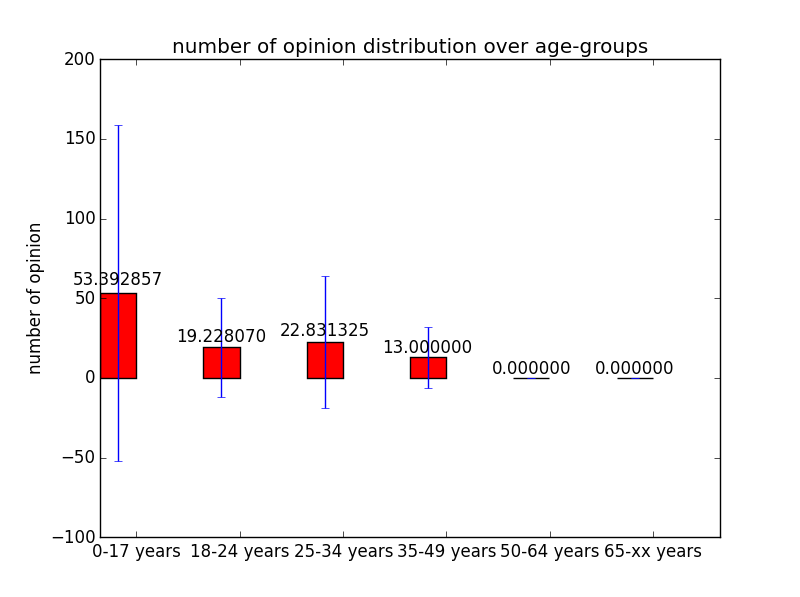
\includegraphics[width=0.5\textwidth]{koppel/age_numopinion.png}%
}%
\end{figure*}

\begin{figure*}
\subfloat[Blog Opinion Score vs Age]{
  \label{fig:Raw_scatter}%
  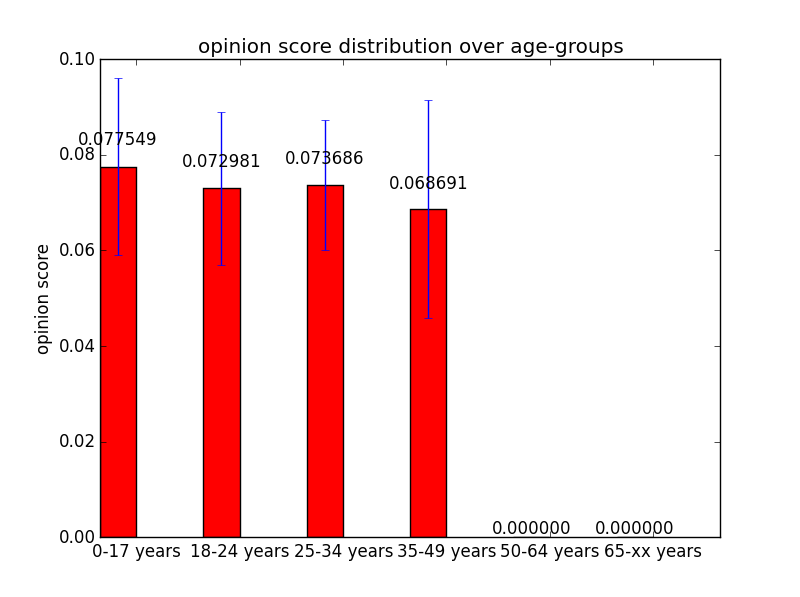
\includegraphics[width=0.5\textwidth]{koppel/age_opinionscore.png}%
}%
\hspace*{\fill}
\subfloat[\# of instances of Character Flooding vs age]{%
  \label{fig:Num_Raw_scatter}%
  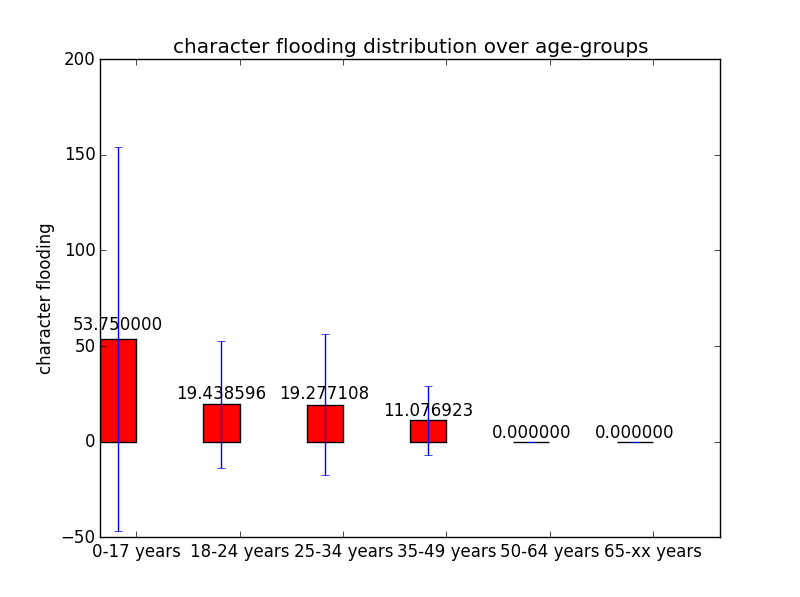
\includegraphics[width=0.5\textwidth]{koppel/age_characterflooding.png}%
}%
\end{figure*}

\begin{figure*}
\subfloat[\# of instances of Character Flooding vs Gender]{
  \label{fig:Total_Raw_scatter}%
  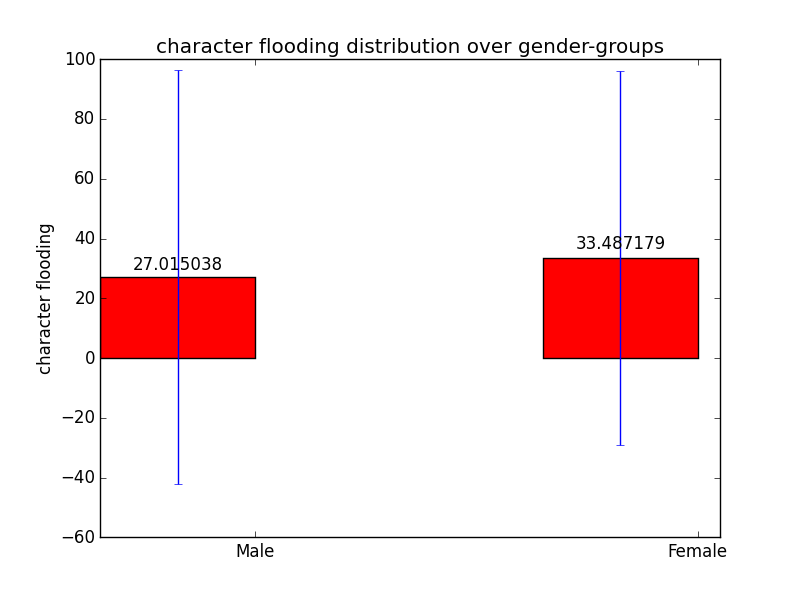
\includegraphics[width=0.5\textwidth]{koppel/gender_characterflooding.png}%
}%
\hspace*{\fill}
\subfloat[\# of Facts vs Gender]{
  \label{fig:Num_Total_scatter}%
  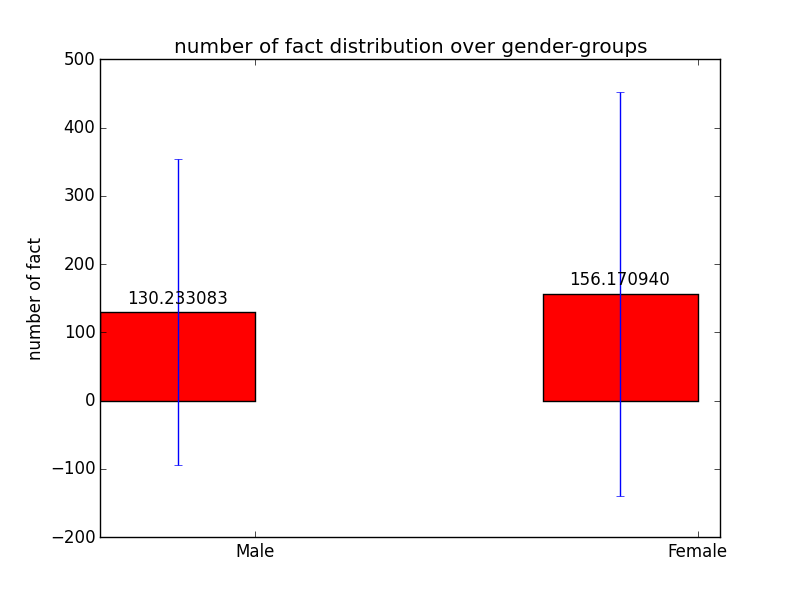
\includegraphics[width=0.5\textwidth]{koppel/gender_numfact.png}%
}%
\end{figure*}

\begin{figure*}
\subfloat[\# of Opinions vs Gender]{%
  \label{fig:Num_Raw_scatter}%
  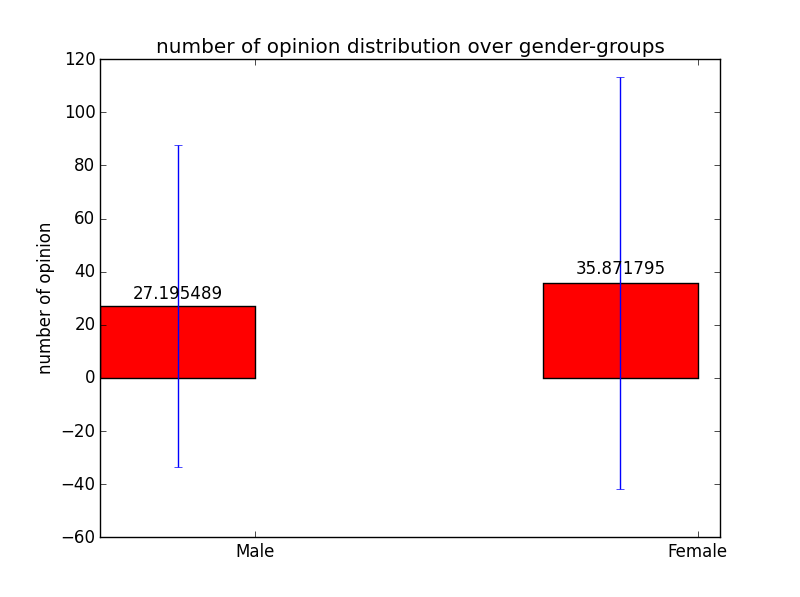
\includegraphics[width=0.5\textwidth]{koppel/gender_numopinion.png}%
}%
\hspace*{\fill}
\subfloat[Blog Opinion Score vs Gender]{
  \label{fig:Total_Raw_scatter}%
  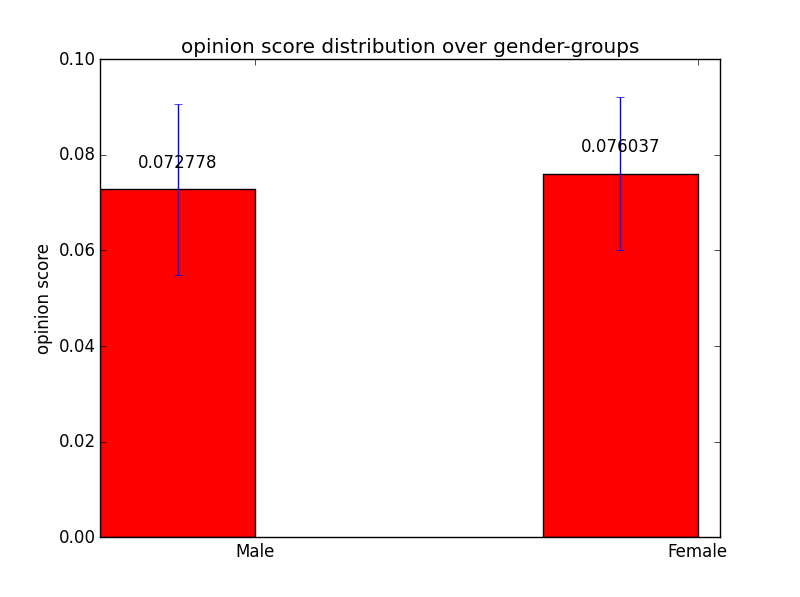
\includegraphics[width=0.5\textwidth]{koppel/gender_opinionscore.png}%
}%
\end{figure*}

\begin{figure*}
\subfloat[\# of instances of Character Flooding vs Age]{
      \label{fig:Num_Total_scatter}%
        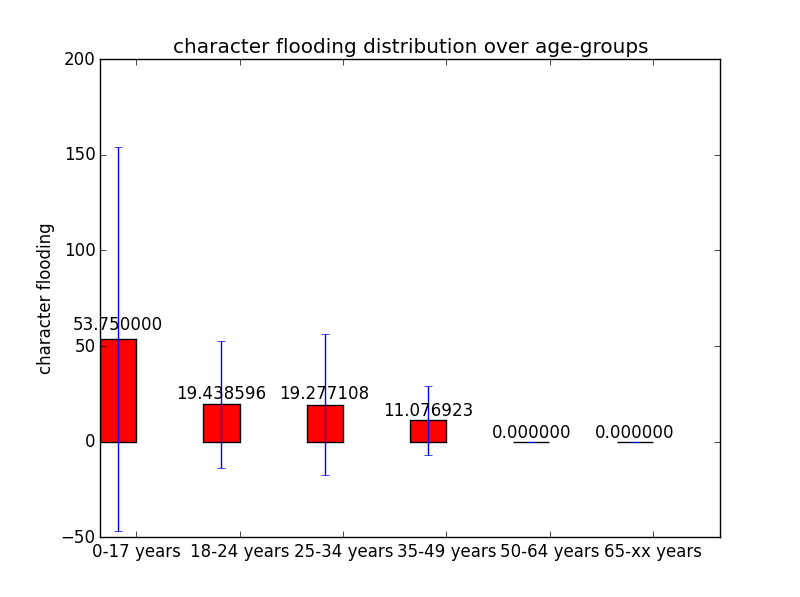
\includegraphics[width=0.5\textwidth]{koppel/age_characterflooding.png}%
}%
\hspace*{\fill}
\subfloat[\# of Facts vs Age]{
      \label{fig:Num_Total_scatter}%
        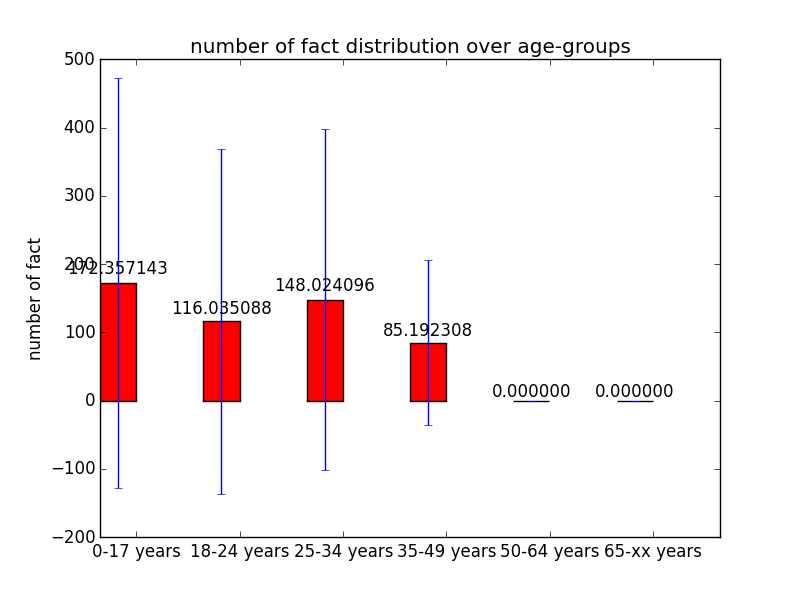
\includegraphics[width=0.5\textwidth]{koppel/age_numfact.png}%
}%
\end{figure*}

\begin{figure*}
\subfloat[\# of opinions vs Age]{
      \label{fig:Num_Total_scatter}%
        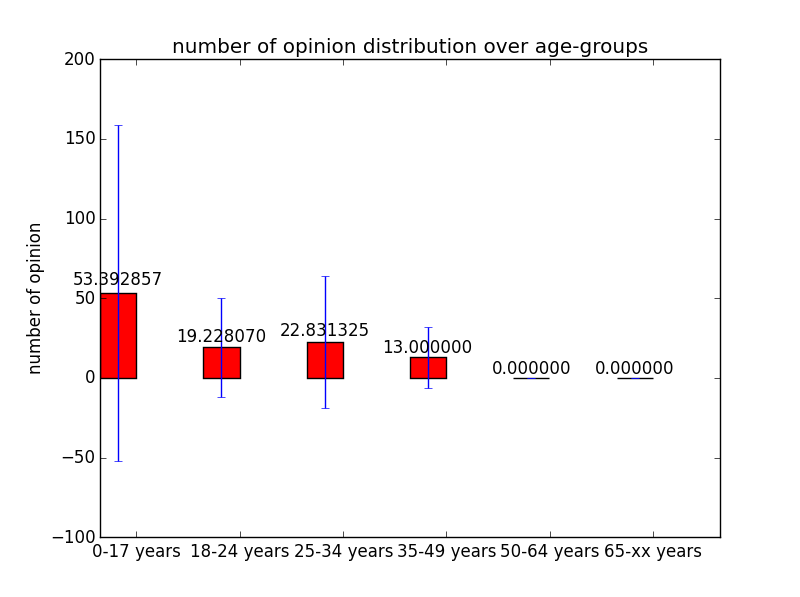
\includegraphics[width=0.5\textwidth]{koppel/age_numopinion.png}%
}%
\hspace*{\fill}
\subfloat[Blog Opinion Score vs Age]{
      \label{fig:Num_Total_scatter}%
        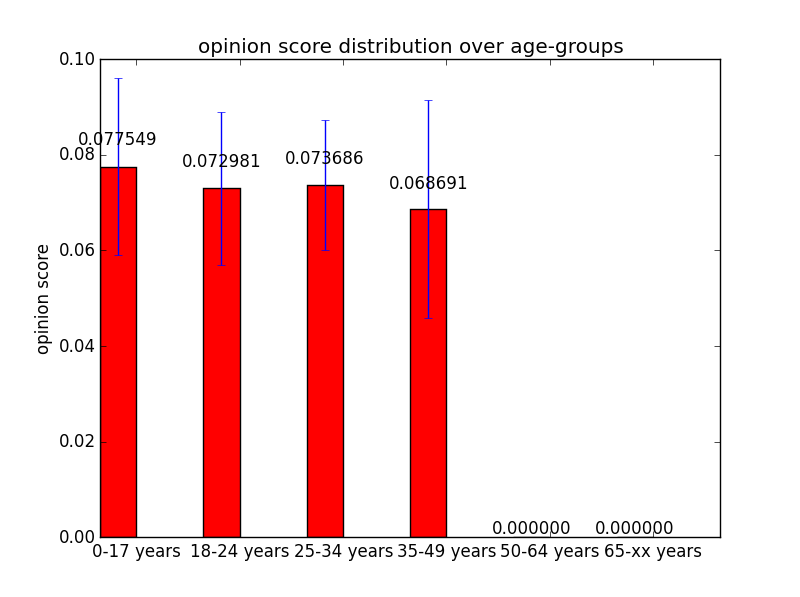
\includegraphics[width=0.5\textwidth]{koppel/age_opinionscore.png}%
}%
\end{figure*}

\begin{figure*}
\subfloat[\# of Inter-sentential Discourse Relations vs Age]{
      \label{fig:Num_Total_scatter}%
        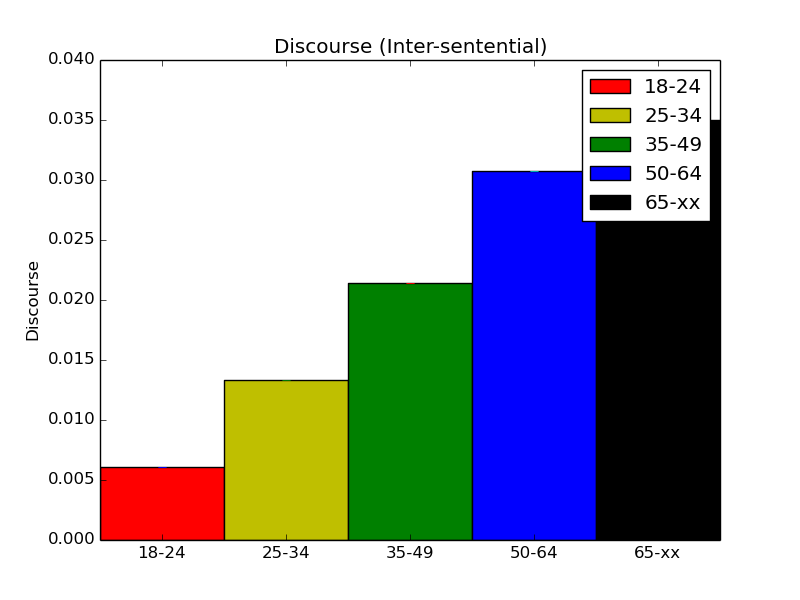
\includegraphics[width=0.5\textwidth]{koppel/Discourse_Age.png}%
}%
\hspace*{\fill}
\subfloat[\# of Inter-sentential Discourse Relations vs Gender]{
      \label{fig:Num_Total_scatter}%
        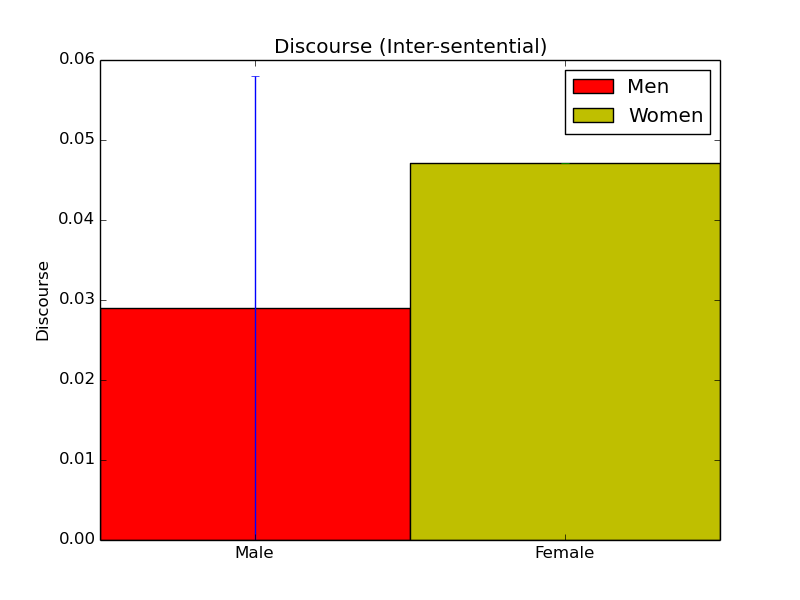
\includegraphics[width=0.5\textwidth]{koppel/Discourse_Gender.png}%
}%
\end{figure*}

\begin{figure*}
\subfloat[\# of instances of Character Flooding vs Gender]{
      \label{fig:Num_Total_scatter}%
        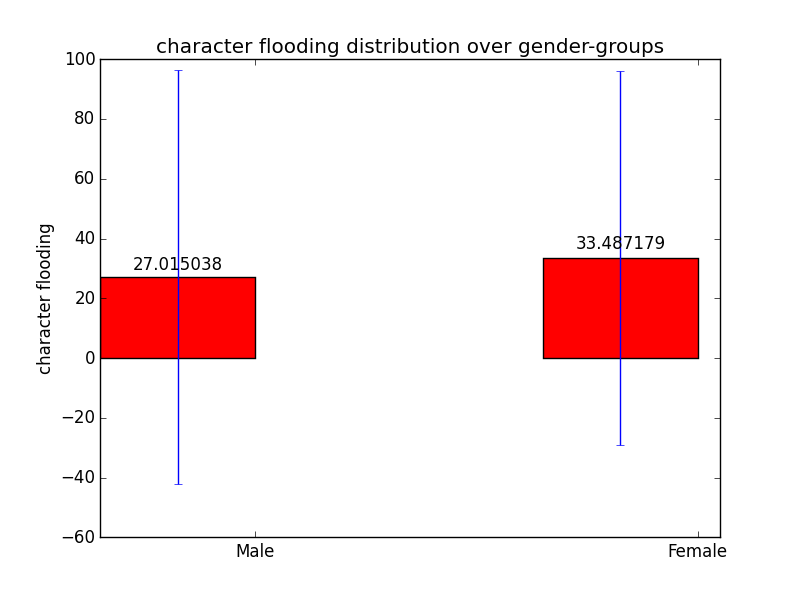
\includegraphics[width=0.5\textwidth]{koppel/gender_characterflooding.png}%
}%
\hspace*{\fill}
\subfloat[\# of Facts vs Gender]{
      \label{fig:Num_Total_scatter}%
        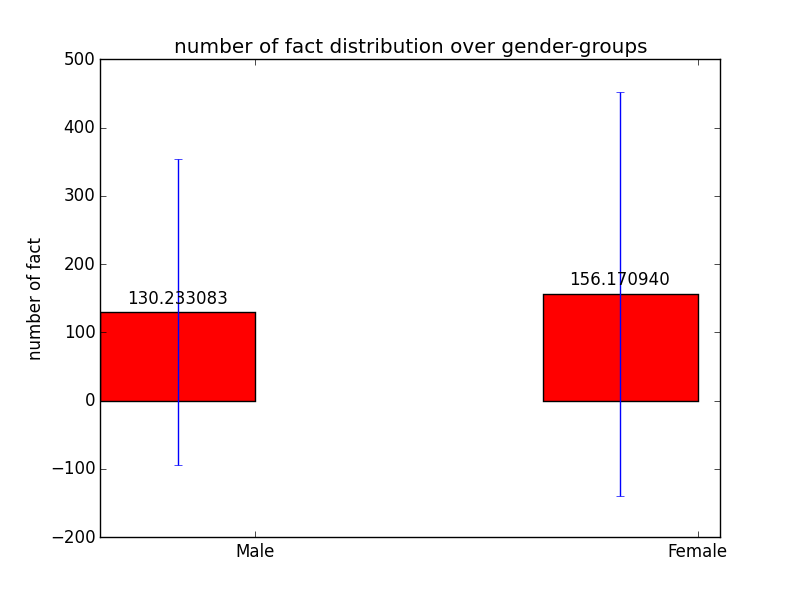
\includegraphics[width=0.5\textwidth]{koppel/gender_numfact.png}%
}%
\end{figure*}

\begin{figure*}
\subfloat[\# of Opinions vs Gender]{
      \label{fig:Num_Total_scatter}%
        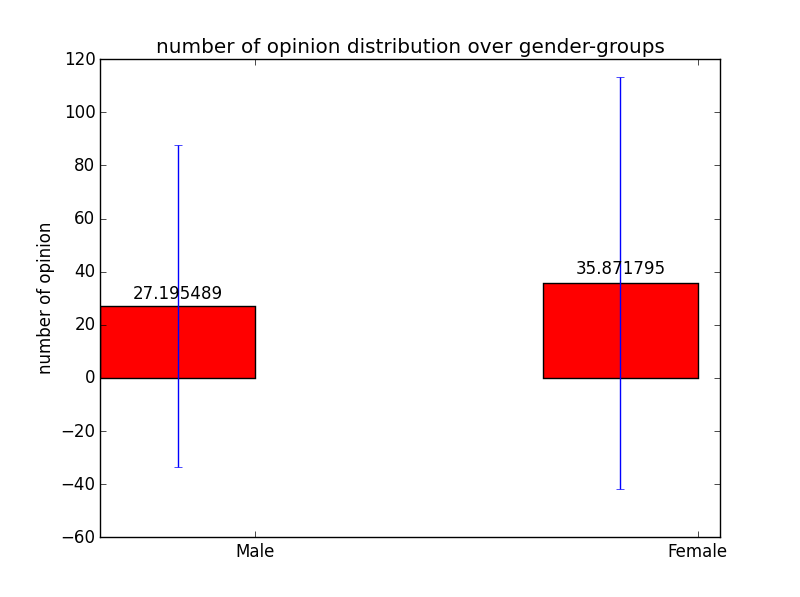
\includegraphics[width=0.5\textwidth]{koppel/gender_numopinion.png}%
}%
\hspace*{\fill}
\subfloat[Blog Opinion Score vs Gender]{
      \label{fig:Num_Total_scatter}%
        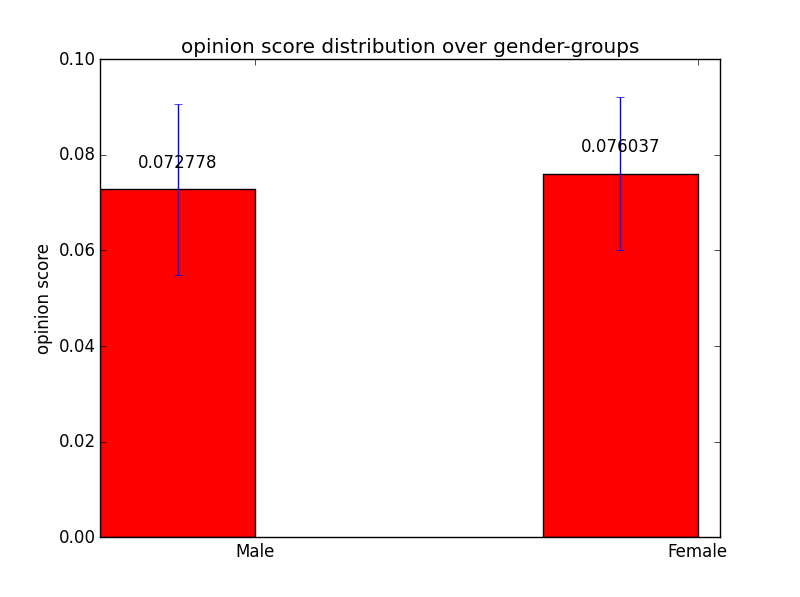
\includegraphics[width=0.5\textwidth]{koppel/gender_opinionscore.png}%
}%
\end{figure*}

\begin{figure*}
\subfloat[Average \# of HTML Links vs Age]{
      \label{fig:Num_Total_scatter}%
        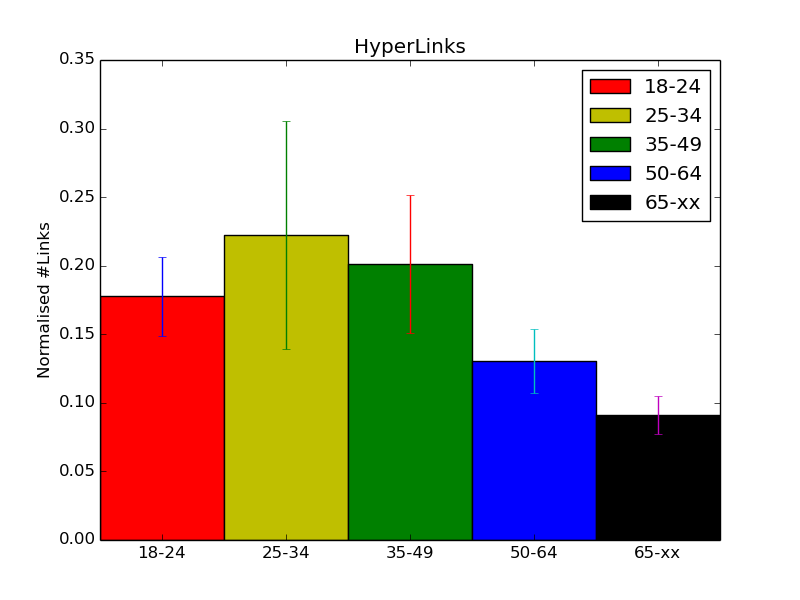
\includegraphics[width=0.5\textwidth]{koppel/Links_Age2.png}%
}%
\hspace*{\fill}
\subfloat[Average \# of HTML Links vs Gender]{
      \label{fig:Num_Total_scatter}%
        \includegraphics[width=0.5\textwidth]{koppel/Links_Gender.png}%
}%
\end{figure*}

\begin{figure*}
\subfloat[Average \# of Named Entities used vs Age]{
      \label{fig:Num_Total_scatter}%
        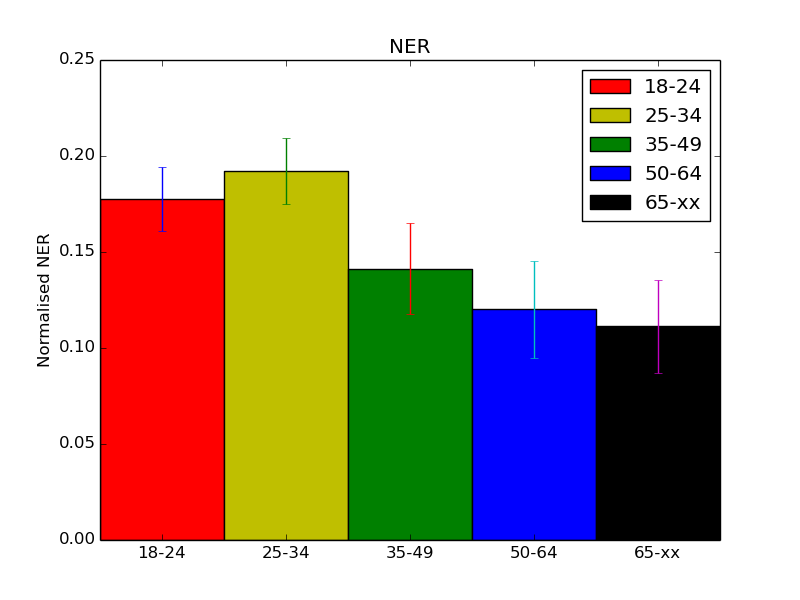
\includegraphics[width=0.5\textwidth]{koppel/NER_Age2.png}%
}%
\hspace*{\fill}
\subfloat[Average \# of Named Entities used vs Age]{
      \label{fig:Num_Total_scatter}%
        \includegraphics[width=0.5\textwidth]{koppel/NER_Age.png}%
}%
\end{figure*}

\begin{figure*}
\subfloat[Average \# of Named Entities used vs Gender]{
      \label{fig:Num_Total_scatter}%
        \includegraphics[width=0.5\textwidth]{koppel/NER_Gender.png}%
}%
\hspace*{\fill}
\subfloat[\# of Non-word Errors vs Age]{
      \label{fig:Num_Total_scatter}%
        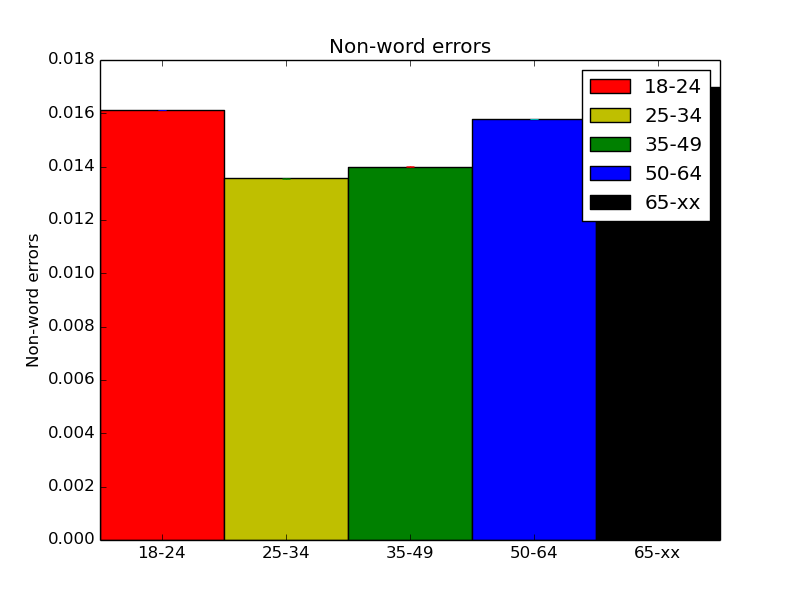
\includegraphics[width=0.5\textwidth]{koppel/Non-worderrors_Age.png}%
}%
\end{figure*}

\begin{figure*}
\subfloat[\# of Non-word Errors vs Gender]{
      \label{fig:Num_Total_scatter}%
        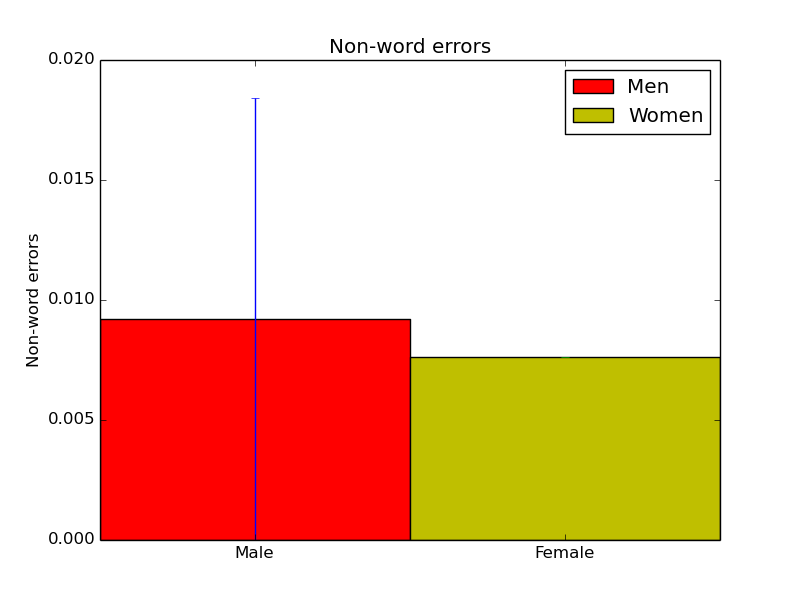
\includegraphics[width=0.5\textwidth]{koppel/Non-worderrors_Gender.png}%
}%
\hspace*{\fill}
\subfloat[Cumulative Distribution of POS tags vs Age]{
      \label{fig:Num_Total_scatter}%
        \includegraphics[width=0.5\textwidth]{koppel/POS_Age.png}%
}%
\end{figure*}

\begin{figure*}
\subfloat[Cumulative Distribution of POS tags vs Gender]{
      \label{fig:Num_Total_scatter}%
        \includegraphics[width=0.5\textwidth]{koppel/POS_Gender.png}%
}%
\hspace*{\fill}
\subfloat[Average Sentence Length vs Age]{
      \label{fig:Num_Total_scatter}%
        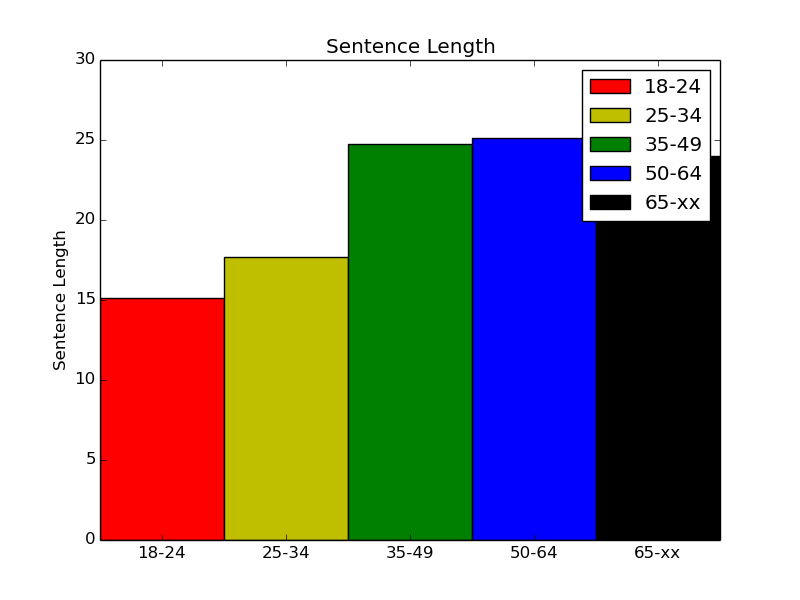
\includegraphics[width=0.5\textwidth]{koppel/SentenceLength_Age2.png}%
}%
\end{figure*}

\begin{figure*}
\subfloat[Average Sentence Length vs Age]{
      \label{fig:Num_Total_scatter}%
        \includegraphics[width=0.5\textwidth]{koppel/SentenceLength_Age.png}%
}%
\hspace*{\fill}
\subfloat[Average Sentence Length]{
      \label{fig:Num_Total_scatter}%
        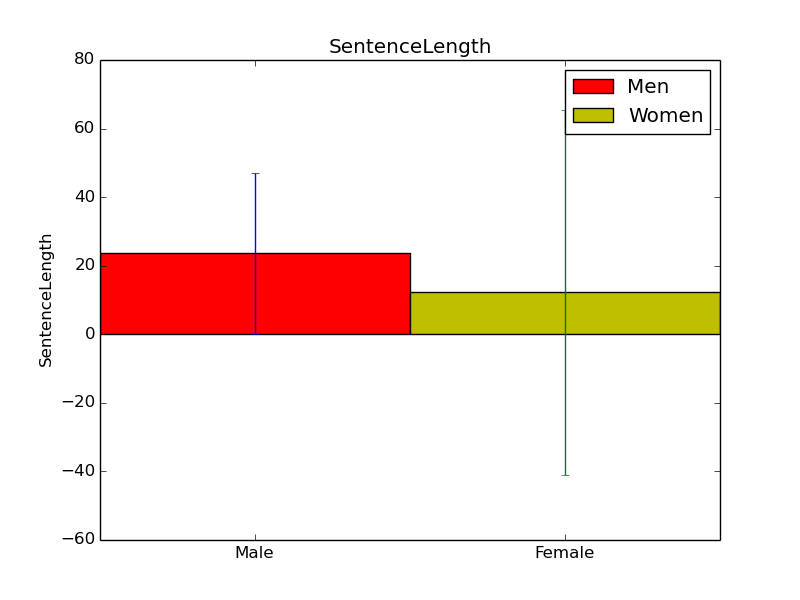
\includegraphics[width=0.5\textwidth]{koppel/sentenceLength.png}%
}%
\end{figure*}

\begin{figure*}
\subfloat[Average \# of Future/Past time references vs Age]{
      \label{fig:Num_Total_scatter}%
        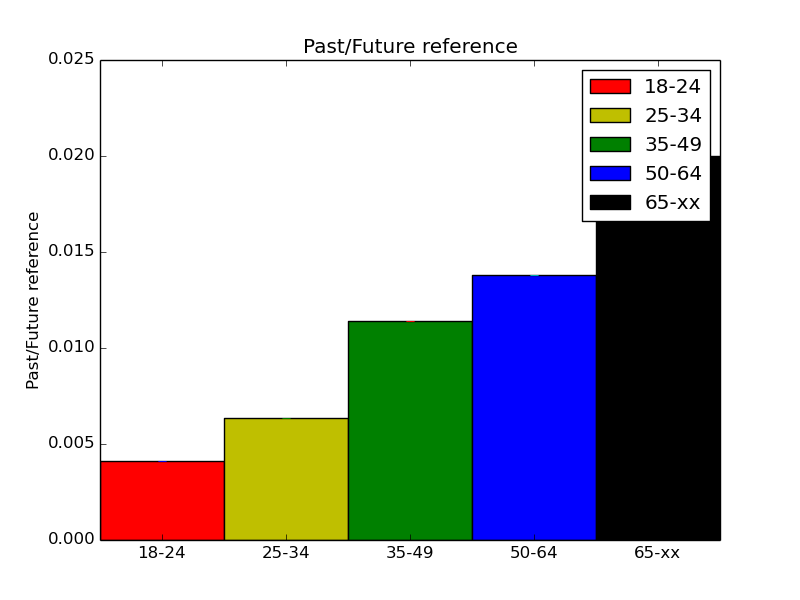
\includegraphics[width=0.5\textwidth]{koppel/timereference_Age.png}%
}%
\hspace*{\fill}
\subfloat[Average \# of Future/Past time references vs Gender]{
      \label{fig:Num_Total_scatter}%
        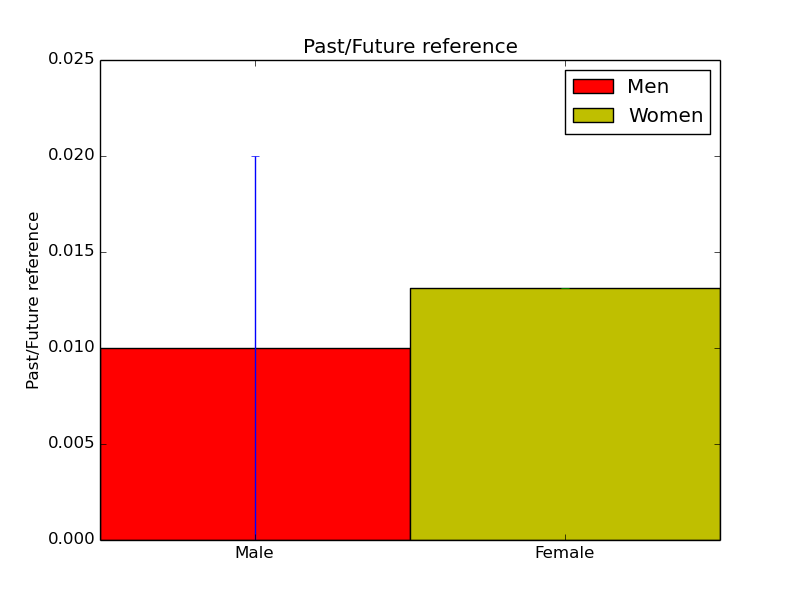
\includegraphics[width=0.5\textwidth]{koppel/timereference_Gender.png}%
}%
\end{figure*}
\pagebreak
\textbf{For Age Bucket Classification:}
\begin{itemize}
\item \# of facts vs Age --- contains average \# of factual blogs vs age buckets 
\item \# of opinions vs Age --- contains average \# of opinion blogs vs age buckets 
\item Blog opinion score vs Age --- contains average blog opinion score vs age buckets
\item \# of instances of character flooding vs Age --- contains average \# of instances of character flooding (like 'hellooo') vs age buckets
\item Average \# of inter-sentential discourse relations vs Age: contains average normalized \# of inter-sentential discourse relations ($X$) vs age buckets
\begin{align}
X = \frac{\# \textrm{of inter-sentential discourse relations in a blog}}{\#\textrm{of sentences in that blog}}
\end{align}
\item Average \# of HTML links vs Age --- contains average normalized \# of HTML links ($X$) vs age buckets
\begin{align}
X = \frac{\# \textrm{of HTML links in a blog}}{\#\textrm{of sentences in that blog}}
\end{align}
\item Average \# of named entities used vs Age--- contains average normalized \# of named entities ($X$) vs age buckets
\begin{align}
X = \frac{\# \textrm{of named entities in a blog}}{\#\textrm{of sentences in that blog}}
\end{align}
\item Average \# of non-word errors vs Age--- contains average normalized \# of non-word errors ($X$) vs age buckets
\begin{align}
X = \frac{\# \textrm{of non-word errors in a blog}}{\#\textrm{of words in that blog}}
\end{align}
\item Distribution of POS tags vs Age --- contains Cumulative Distribution of usage of POS tags vs age buckets
\item Average sentence length vs Age: contains average sentence length vs age buckets 
\item Average \# of future/past time references vs Age --- contains average normalized \# of future/past time references ($X$) vs age buckets
\begin{align}
X = \frac{\# \textrm{of future/past time references in a blog}}{\#\textrm{of sentences in that blog}}
\end{align}
\end{itemize}
\textbf{For Gender Classification:}
Similar plots, as for Age Bucket Classification.
\subsection{PAN'14 Corpus}
Here is the description about plots obtained from PAN'14 Corpus.\\

\begin{figure*}
\subfloat[\# of HTML Links vs Age]{%
  \label{fig:Total_scatter}%
  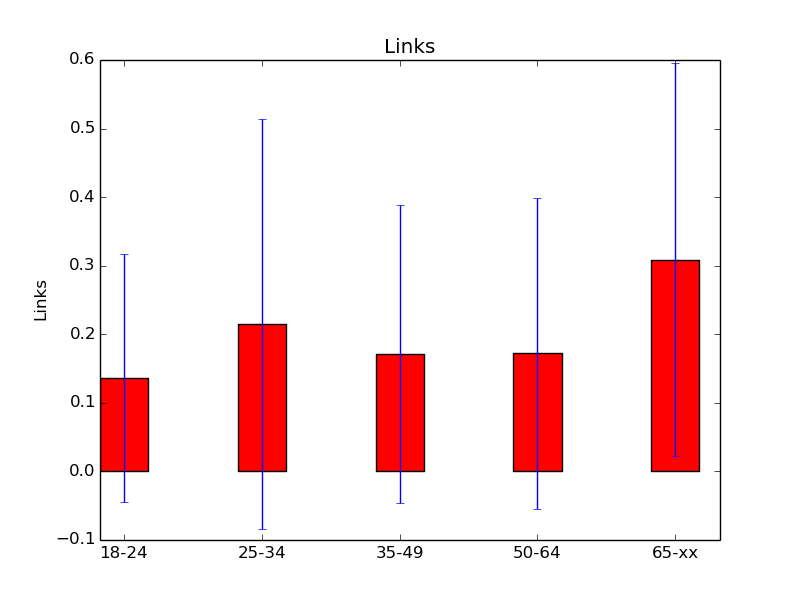
\includegraphics[width=0.5\textwidth]{pan/Links_Age.png}%
}%
\hspace*{\fill}
\subfloat[Average Sentence Length vs Age]{
  \label{fig:Total_Raw_scatter}%
  \includegraphics[width=0.5\textwidth]{pan/SentenceLength_Age.png}%
}%
\end{figure*}
\begin{figure*}
\subfloat[\# of Named Entities used vs Gender]{%
  \label{fig:Num_Raw_scatter}%
  \includegraphics[width=0.5\textwidth]{pan/NER_Gender.png}%
}%
\hspace*{\fill}
\subfloat[Average Sentence Length vs Gender]{
  \label{fig:Num_Total_scatter}%
  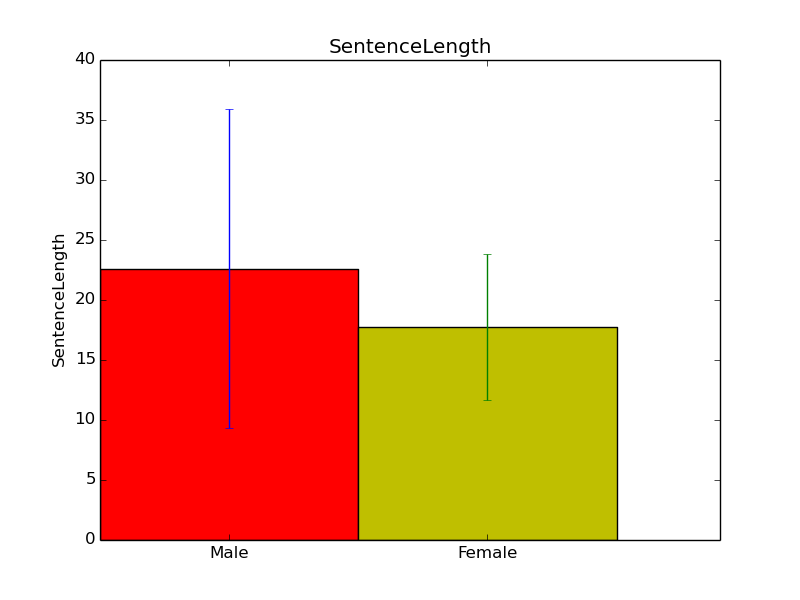
\includegraphics[width=0.5\textwidth]{pan/SentenceLength_Gender.png}%
}
%
\end{figure*}
\begin{figure*}
\subfloat[\# of Named Entities used vs Age]{
  \label{fig:Raw_scatter}%
  \includegraphics[width=0.5\textwidth]{pan/NER_Age.png}%
}
%
\hspace*{\fill}
\subfloat[\# of HTML Links vs Gender]{
  \label{fig:Num_scatter}%
  \includegraphics[width=0.5\textwidth]{pan/Links_Gender.png}%
}
%
\end{figure*}

\begin{figure*}
\subfloat[\# of Quotations vs Age]{
  \label{fig:Raw_scatter}%
  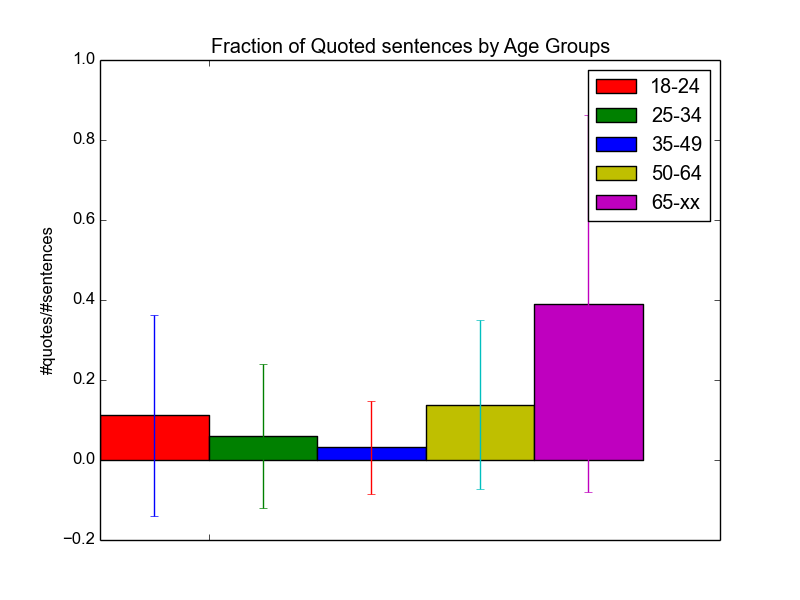
\includegraphics[width=0.5\textwidth]{pan/Fraction_of_Quoted_sentences_by_Age_Groups.png}%
}
%
\hspace*{\fill}
\subfloat[\# of Quotations vs Gender]{
  \label{fig:Num_scatter}%
  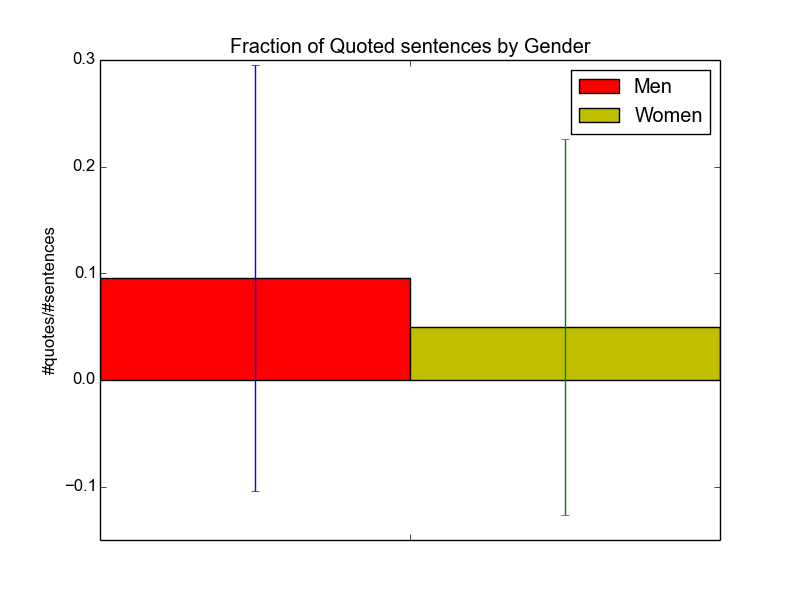
\includegraphics[width=0.5\textwidth]{pan/Fraction_of_Quoted_sentences_by_Gender.png}%
}
%
\end{figure*}

\begin{figure*}
\subfloat[\# of Named Entities used vs Age]{
  \label{fig:Raw_scatter}%
  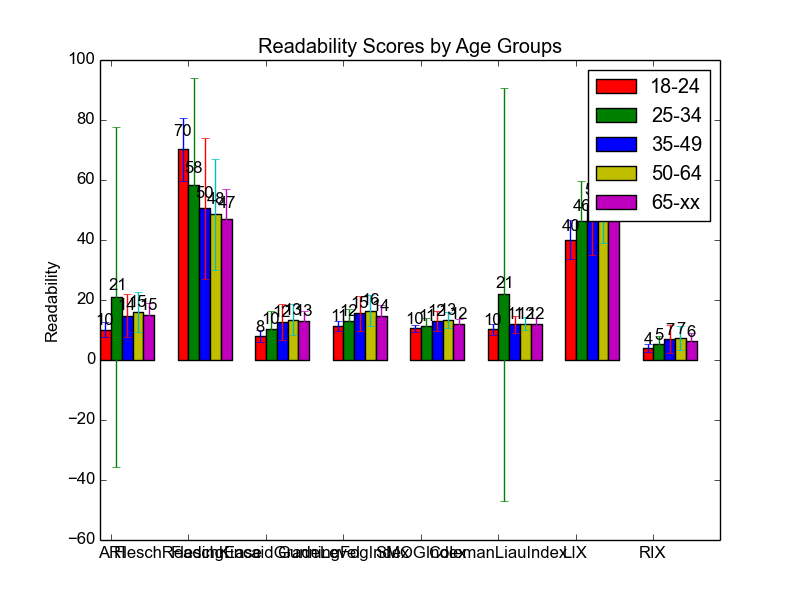
\includegraphics[width=0.5\textwidth]{pan/Readability_Scores_by_Age_Groups.png}%
}
%
\hspace*{\fill}
\subfloat[\# of HTML Links vs Gender]{
  \label{fig:Num_scatter}%
  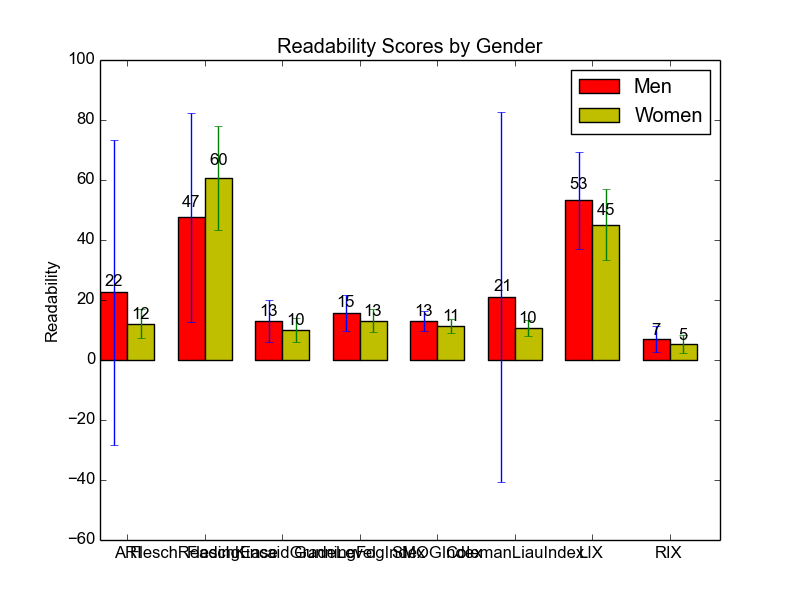
\includegraphics[width=0.5\textwidth]{pan/Readability_Scores_by_Gender.png}%
}
%
\end{figure*}

%\begin{figure*}
%\includegraphics[width=18cm]{pan/POS_Age.png}
%\includegraphics[width=18cm]{pan/POS_Gender.png}
%\caption{Counts of various POS tags in PAN '14 Corpus}
%\end{figure*}

\begin{figure*}
\subfloat[Cumulative Distribution of POS tags vs Gender]{
    \label{fig:Num_scatter}%
	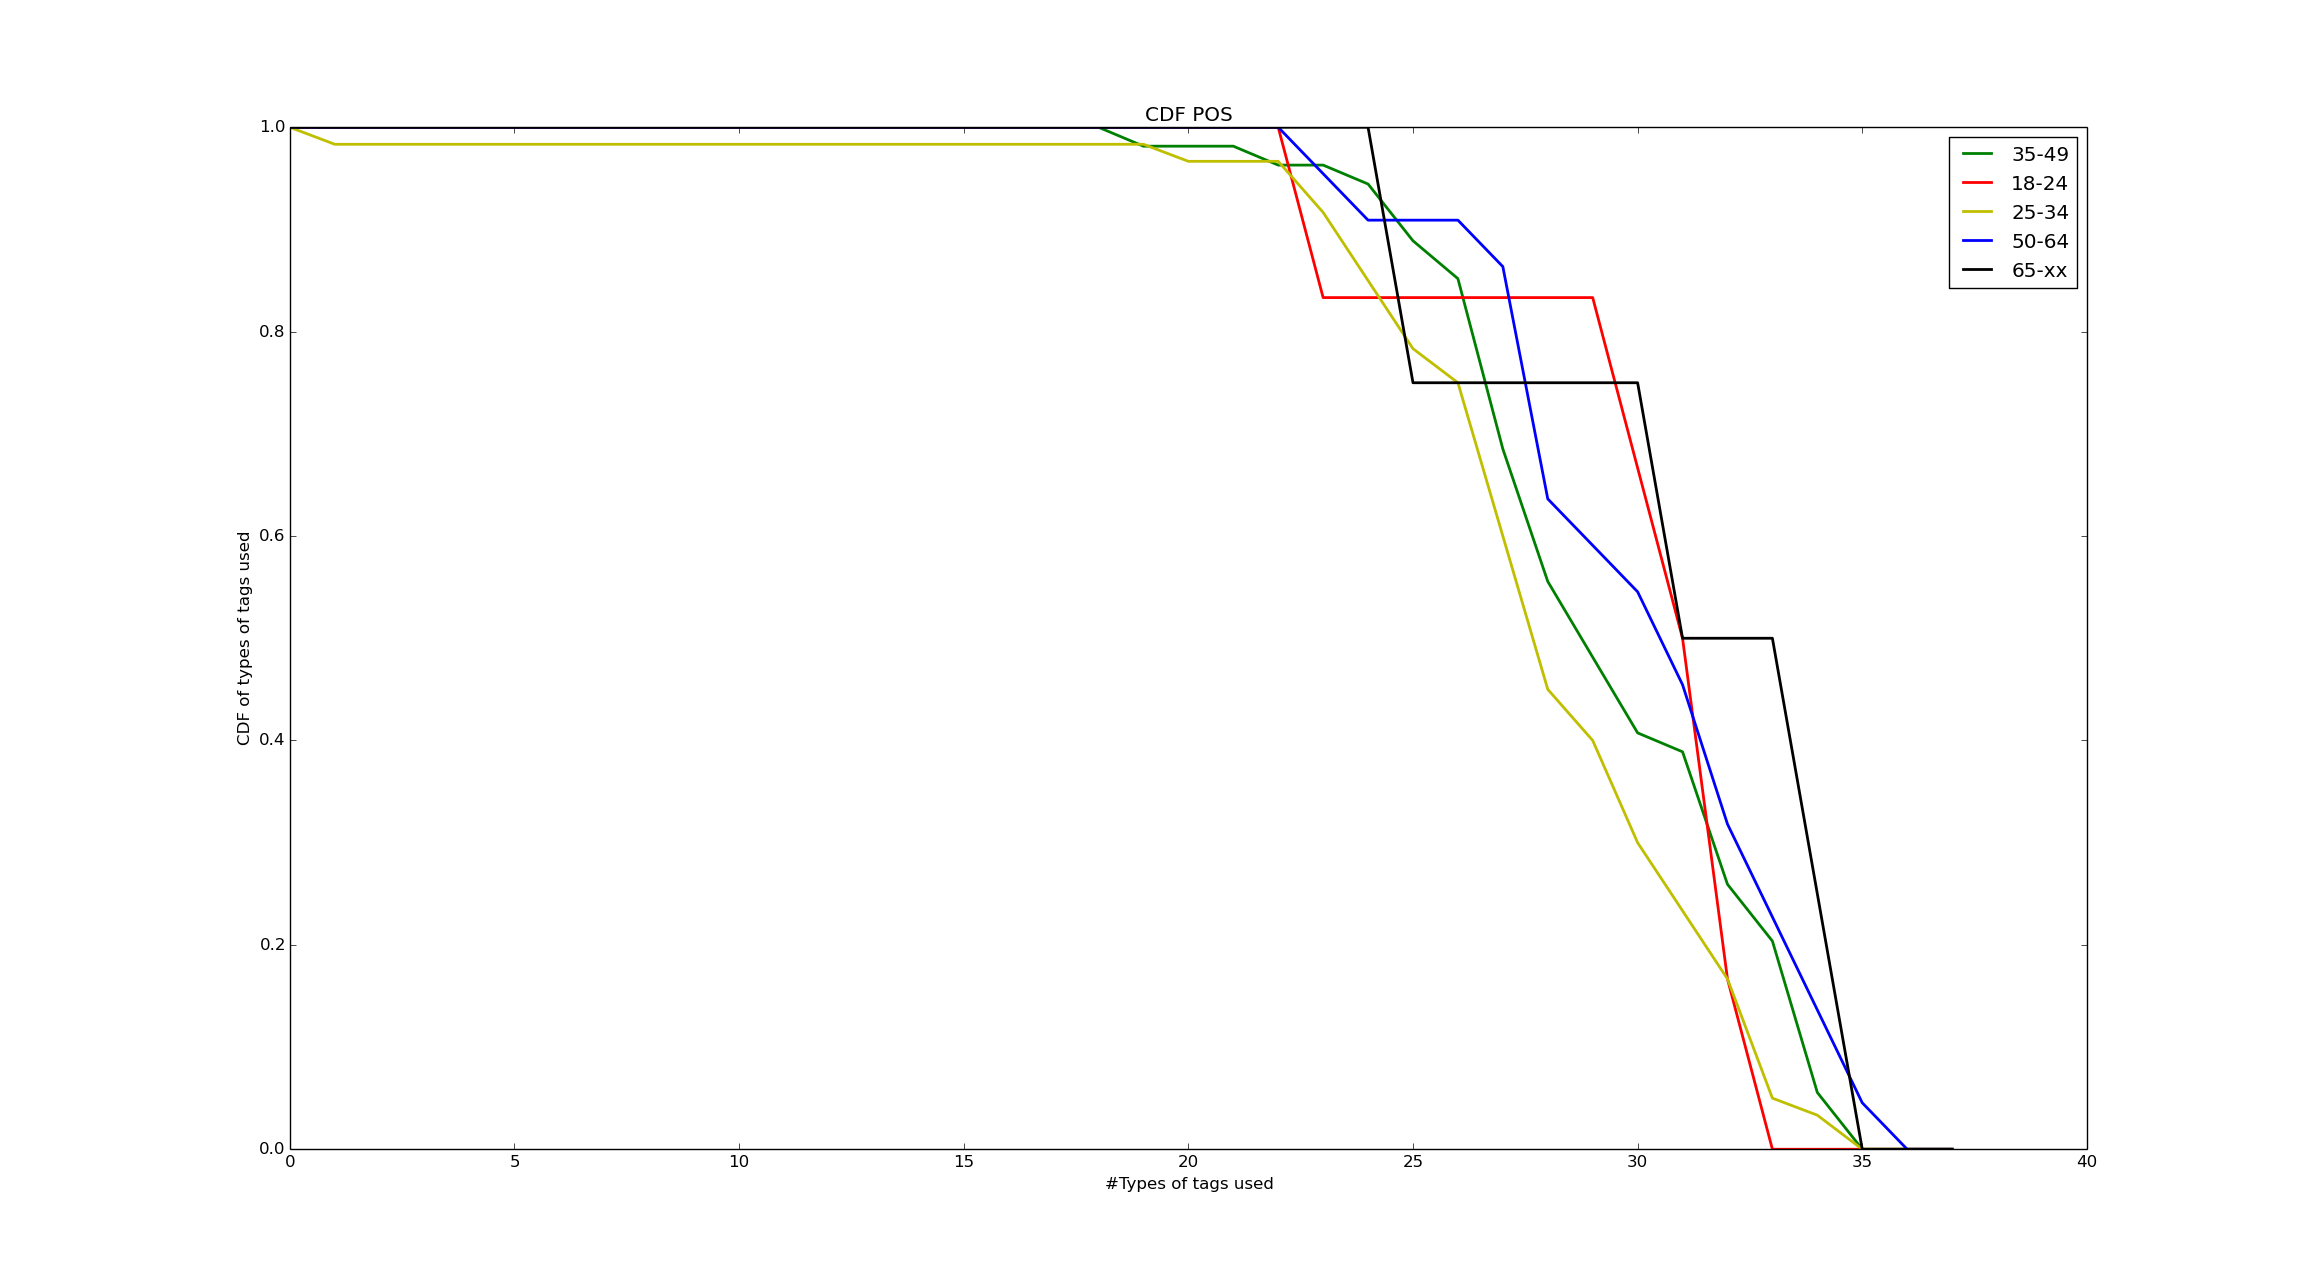
\includegraphics[width=0.5\textwidth]{pan/POS_CDF.png}%
}%
\hspace*{\fill}
\subfloat[Cumulative Distribution of POS tags vs Age]{
    \label{fig:Num_scatter}%
	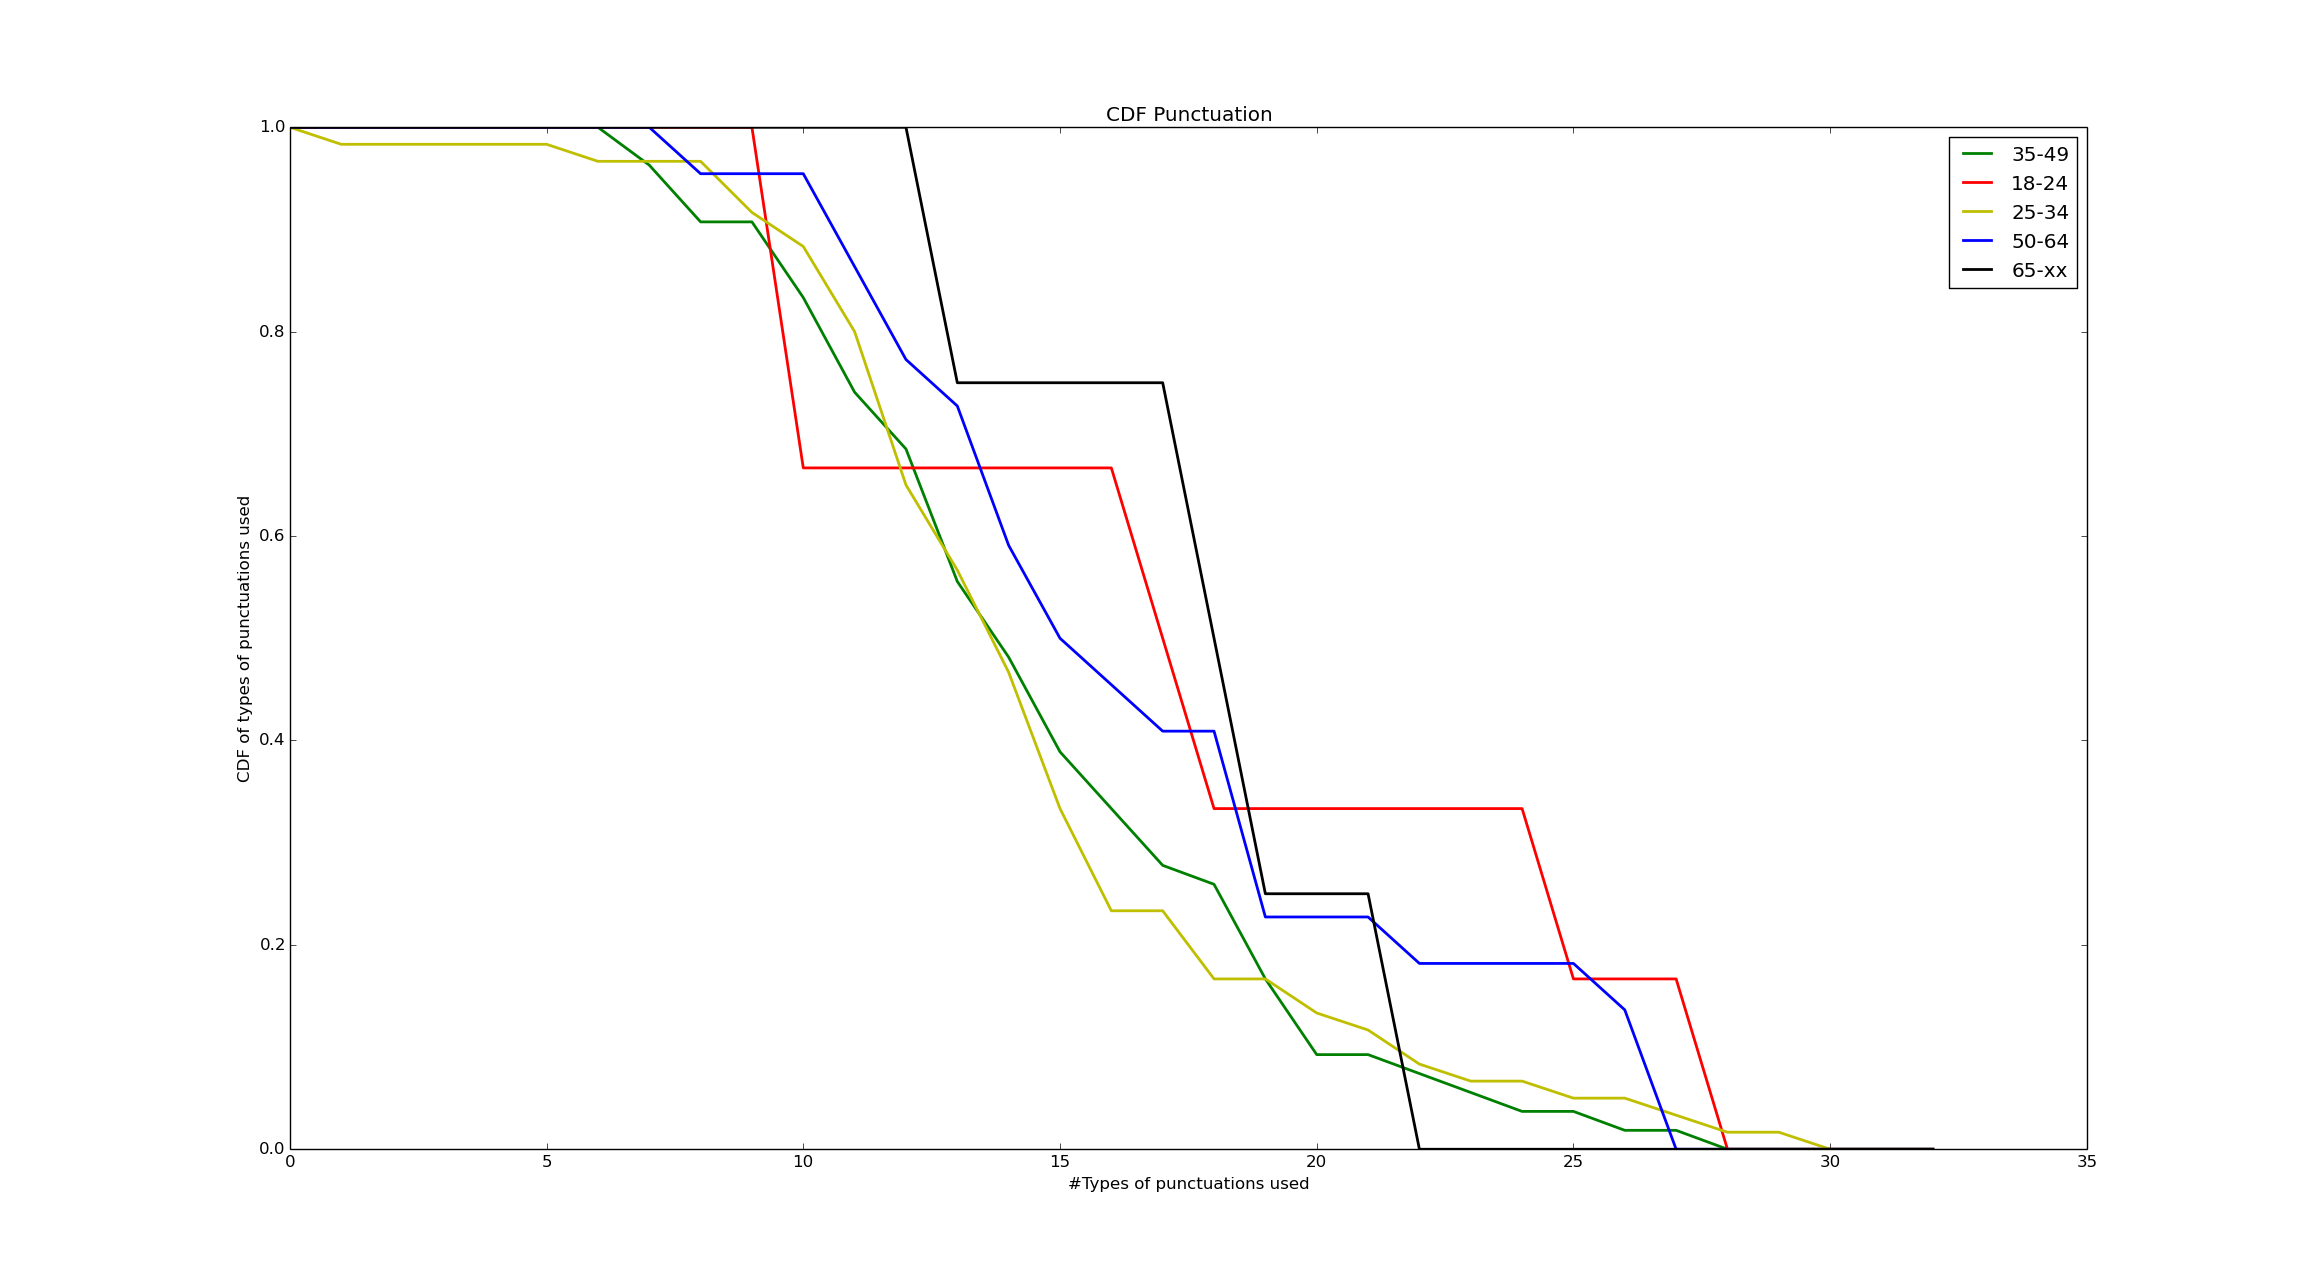
\includegraphics[width=0.5\textwidth]{pan/Punctuation_Age_CDF.png}%
}%
\end{figure*}

%\begin{figure*}
%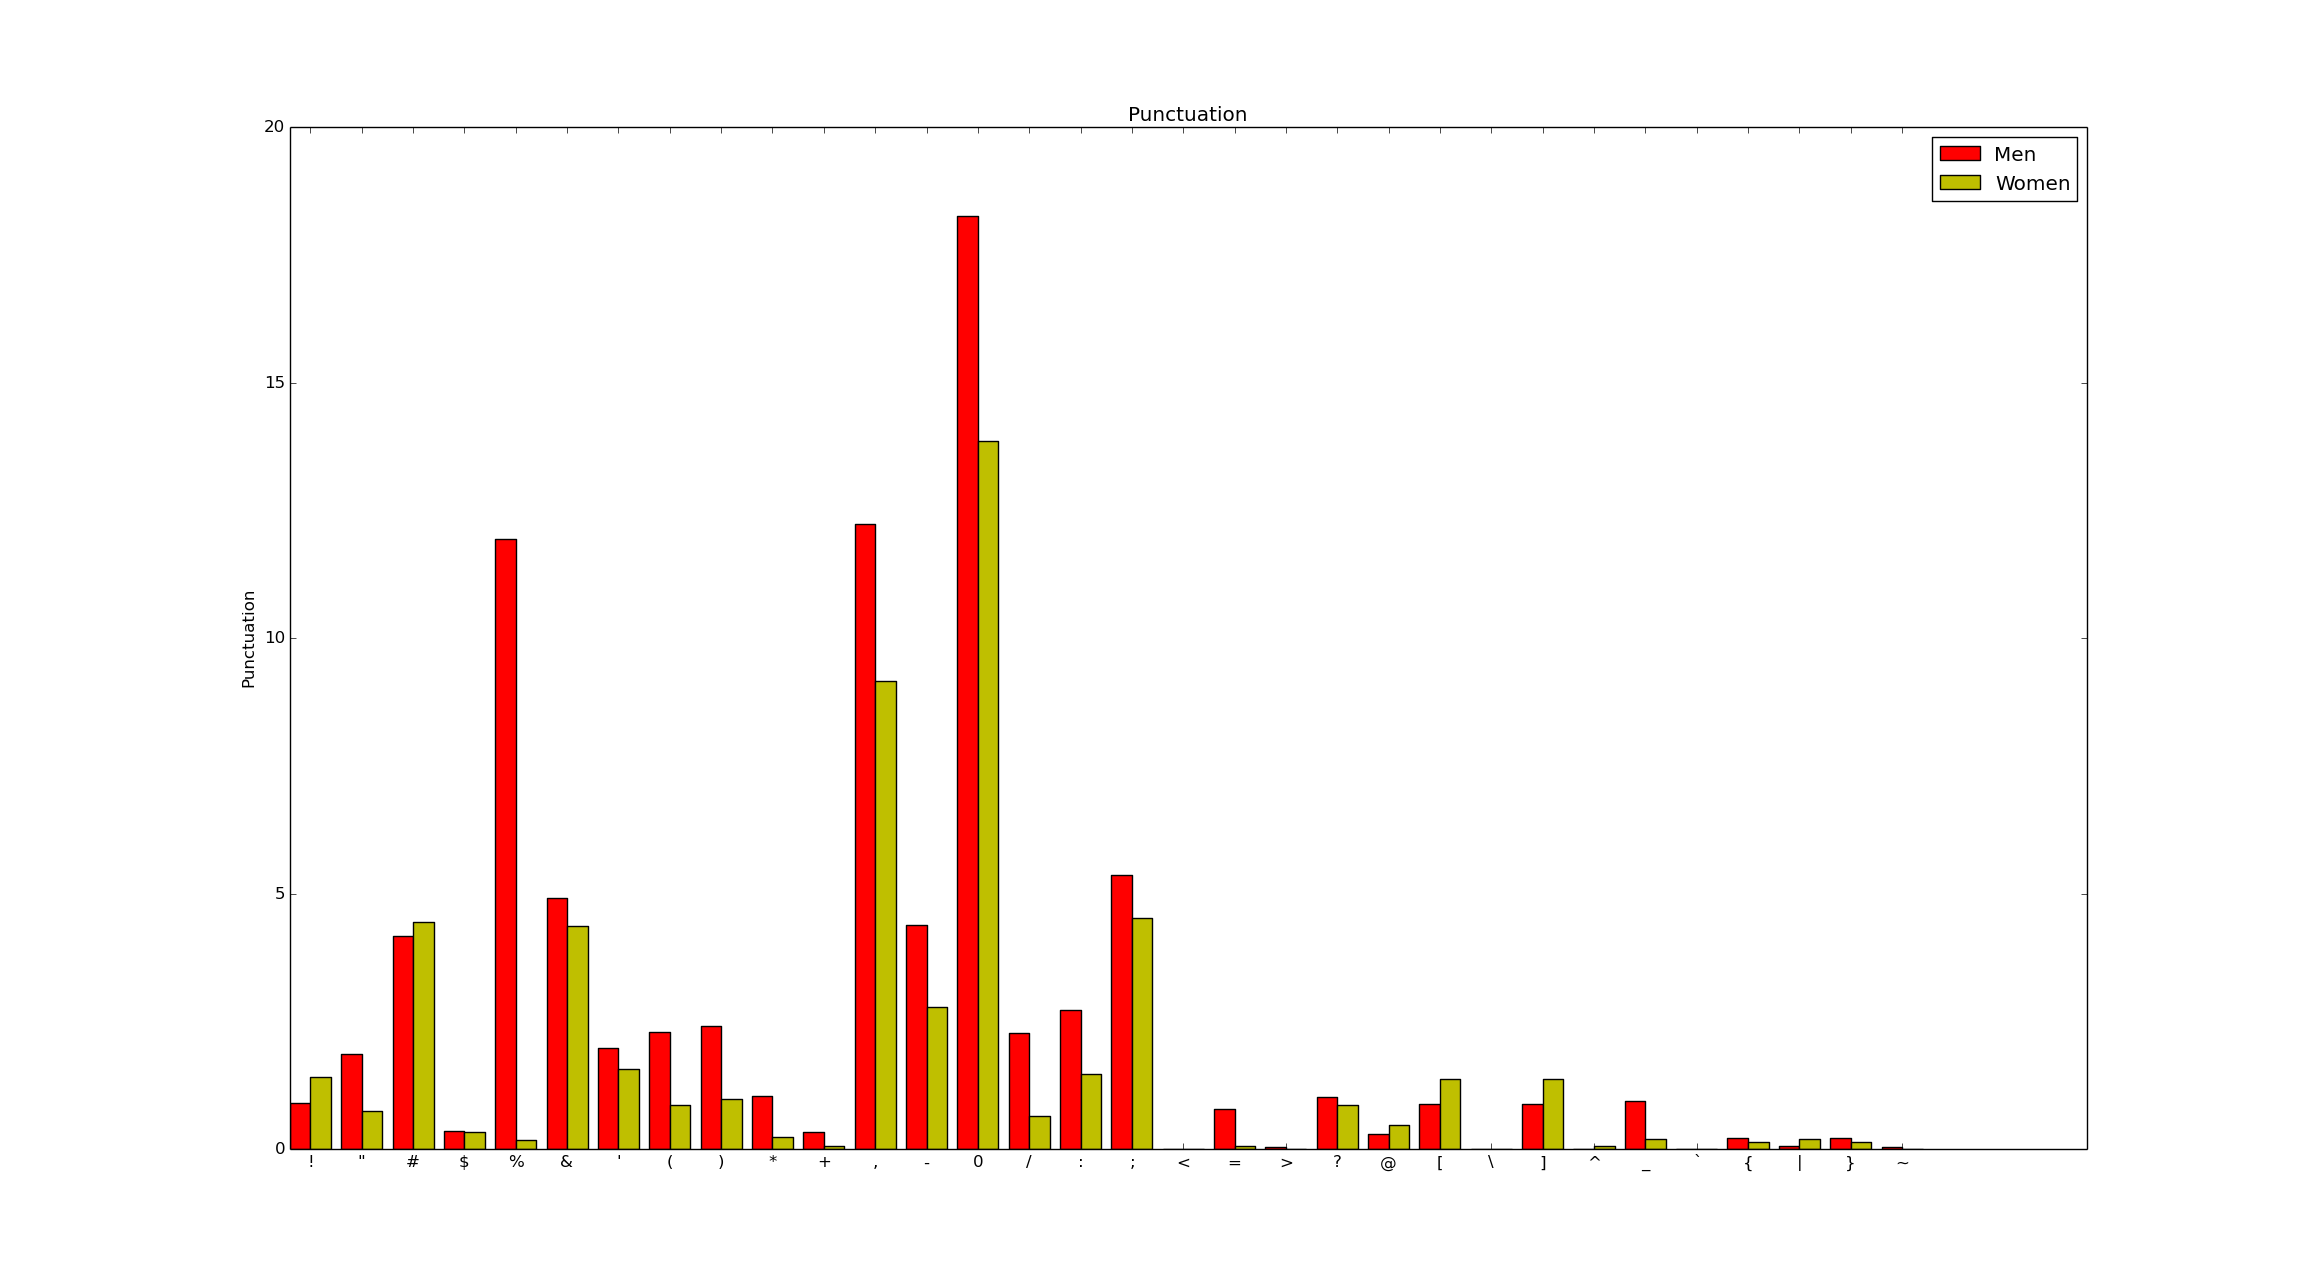
\includegraphics[width=18cm]{pan/Punctuation_Gender.png}
%\caption{Counts of various Punctuation tags in PAN '14 Corpus}
%\end{figure*}

\textbf{For Age Bucket Classification:}
\begin{itemize}
\item Average \# of HTML links vs Age --- contains average normalized \# of HTML links ($X$) vs age buckets
\begin{align}
X = \frac{\# \textrm{of HTML links in a blog}}{\#\textrm{of sentences in that blog}}
\end{align}
\item Average \# of named entities used vs Age--- contains average normalized \# of named entities ($X$) vs age buckets
\begin{align}
X = \frac{\# \textrm{of named entities in a blog}}{\#\textrm{of sentences in that blog}}
\end{align}
\item Distribution of POS tags vs Age --- contains Cumulative Distribution of usage of POS tags vs age buckets
\item Average sentence length vs Age: contains average sentence length vs age buckets 
\item Average \# of quotations vs Age--- contains average normalized \# of quotations ($X$) vs age buckets
\begin{align}
X = \frac{\# \textrm{of quotations in a blog}}{\#\textrm{of sentences in that blog}}
\end{align}
\item Various Readability Scores vs Age --- We computed several readability metrics \textit{[3.2]} like Automated Readability Index(ARI), Flesch Reading Ease, Flesch Kincaid Grade Level, Gunning Fog Index, SMOG Index, Coleman Liau Index, LIX and RIX for the blogs; It is found that as age increases, readability of the text written by that person decreases. This aligns with our intuition. For gender, blogs written by males tend to have less readability that than female authors. 
\end{itemize}

\textbf{For Gender Classification:}
Similar plots, as for Age Bucket Classification.\\
\section{Future Work-plan}
\subsection{Feature Selection}
We shall try using both the techniques for Feature Selection namely --- Feature Subset Selection (FS) using Filters/Wrappers and Dimensionality Reduction (DR) using PCA. The primary focus will be on using Filters for Feature Selection task using Information Gain (IG), as quoted earlier in \textit{[3.3]}.
\subsection{Incorporate Semantic Features}
We expect semantic-based features to add to the performance of the classifier because of the following reasons: 1) Content-based or Style-based features alone do not consider the semantic relation between words. 2) These do not handle polysemy. \cite{iiit_god} shows that classifiers learned using semantic features based on Wikipedia Category Information achieve significantly better accuracy compared to the state-of-the-art methods. Hence, we aim to cover this and other semantic features in our classifier as well.
\subsection{Deep Learning}
Deep Learning techniques have proven themselves to have an astonishing performance over the conventional methods. Using Word2Vec, we shall try incorporating deep learning approach for out task and evaluate its performance vs the state-of-the-art methods.
\subsection{Regression Modeling}
With reference to the regression model discussed in this study --- \cite{cmu}, we will compare the performance of the regression approach for modeling the age of the author vs our classification approach to identify the age bucket. 

\section{Performance Evaluation}
For the Blog Authorship Corpus, we plan to use k-Fold Cross Validation for evaluation of classifiers, as quoted in \textit{[3.4]}.
For the PAN'14 Corpus, we have a test data-set (corresponding to PAN' 15) which is unlabeled and the tagged data-set will be released in recent future. If we don't get access to that soon, we will go with k-Fold Cross Validation on the PAN' 14 data. 
\newpage
\begin{thebibliography}{9}
\bibitem{arbit} 
James Marquardt et al.
[\textit{Age and Gender Identication in Social Media}]. 
Annalen der Physik, 322(10):891–921, 1905.

\bibitem{iiit-god} 
K Santosh, Romil Bansal, Mihir Shekhar, and Vasudeva Varma
\textit{Exploiting Wikipedia Categorization for Predicting Age
and Gender of Blog Authors}. 
Notebook for PAN at CLEF 2013.

\bibitem{cmu} 
Dong Nguyen, Noah A. Smith, and Carolyn P. Rosé
\textit{Author Age Prediction from Text using Linear Regression}. 
In Proceedings of the ACL Workshop on Language Technology for Cultural Heritage, Social Sciences, and Humanities (LATECH 2011), Portland, OR, June 2011.

\bibitem{pan} 
Francisco Rangel, Paolo Rosso, Moshe Koppel, Efstathios Stamatatos, and Giacomo Inches. \textit{Overview of the Author Profiling Task at PAN 2013}. 
Proceedings of PAN at CLEF 2013.

\bibitem{koppel} 
S. Argamon, M. Koppel, J. Pennebaker and J. Schler (2009) 
\textit{Automatically profiling the author of an anonymous text}. 
Communications of the ACM 52 (2): 119–123.

\bibitem{koppel1} 
J. Schler, Moshe Koppel, S. Argamon and J. Pennebaker (2006)
\textit{Effects of Age and Gender on Blogging} 
in Proc. of AAAI Spring Symposium on Computational Approaches for Analyzing Weblogs, March 2006.

\bibitem{mit} 
Andreas Janecek, Wilfried Gansterer, Michael Demel, Gerhard Ecker
\textit{On the Relationship Between Feature Selection and Classification Accuracy} 
JMLR W\&P 4:90-105, 2008.

\end{thebibliography}

\section{Appendix}
Last Page
\end{document}
